%%%
%%% Hauptdokument
%%%

\documentclass[
	a4paper,     		%% Papiergroesse: A4
	twoside,     		%% Zweiseitiges Layout (alternativ: oneside)
	headsepline, 		%% Horizontale Linie unter Kopfzeile
	footsepline, 		%% Horizontale Linie ueber Fusszeile
	titlepage,   		%% Eigenstaendige Titelseite (alternativ: notitlepage)
	%halfparskip, 		%% Halbe Leerzeile zwischen zwei Abschnitten (alternativ: parskip, ...)
	12pt,        		%% Schriftgroesse: 12pt (alternativ: 10pt, 11pt, ...)
	bibtotoc,				%% Bilbiographie in's Inhaltsverzeichnis aufnehmen
	liststotoc,			%% Indexe in's Inhaltsverzeichnis aufnehmen
%	smallheadings,	%% Kleine Ueberschriften
%	DIV1,						%% Divisor, Zeilenl�nge ca. 70 Zeichen
	BCOR01cm,				%% Bindekorrektur
%	draft			  		%% Entwurfsmodus, volle/leere Boxen markieren
%	abstracton			%% Titel "`Zusammenfassung"' einschalten
]{scrreprt}

%%%
%%% Pakete
%%%

%%% Glossar
\usepackage[german]{gloss}
\newcommand{\acr}[1]{{\small\gloss[word]{#1}}}

\newcommand{\abk}[1]{#1\xdot}
\DeclareRobustCommand\xdot{\futurelet\token\Xdot}
\def\Xdot{\ifx\token\bgroup.\else\ifx\token\egroup.\else
  \ifx\token\/.\else\ifx\token\ .\else\ifx\token!.\else
  \ifx\token,.\else\ifx\token:.\else\ifx\token;.\else
  \ifx\token?.\else\ifx\token/.\else\ifx\token'.\else
  \ifx\token).\else\ifx\token-.\else\ifx\token+.\else
  \ifx\token~.\else
  \ifx\token.\else.\ \fi\fi\fi\fi\fi\fi\fi\fi\fi\fi\fi\fi\fi\fi\fi\fi} 
\newcommand{\zB}{\mbox{z.\,B}\xdot}

%%% Literaturverzeichnis, deutschen Stil benutzen (dinat)
\usepackage[square]{natbib}
\citestyle{dinat}

%%% Grafik
\usepackage{pstricks}

%%% UML
%\usepackage{pst-node}
%\usepackage{pst-uml}
%\let\umlClass\pstumlClass	%%% workaround: pst-uml und uml kollidieren
%\usepackage{uml}

%%% Deutsche Sprache verwenden
\usepackage{ngerman}

%%% Kodierung der Eingabezeichen setzen (fuer dt. Umlaute etc.)
\usepackage[ansinew]{inputenc}

%%% Zeichen-Kodierung in PDF-Dokumenten
\usepackage[T1]{fontenc}
%\usepackage{ae,aecompl}

%%% Web-Addressen auch mit T1-Encoding
\usepackage[T1]{url}
%%% ... und in tt-Font
\urlstyle{tt}

%%% amsmath, amssymb, amstext: Unterstuetzung div. mathematischer Zeichen etc.
\usepackage{amsmath,amssymb,amstext}

%%% pifont: "pifont Xs and Check Marks"
\usepackage{pifont}

%%% PostScript-Fonts ersetzen
\usepackage{psfrag}

%%% Programmcode einbinden, Listings
\usepackage{listings}

%%% Farb-Unterstuetzung
\usepackage{color}

%%% Tabellen
\usepackage{booktabs}
\usepackage{array}
\usepackage{multirow}
\usepackage{tabularx}
\usepackage{threeparttable}	% Fussnoten in table-Umgebung

%%% Floats strikter positionieren (Option 'H'ere)
\usepackage{float}

%%%
%%% Pakete konfigurieren, Definitionen
%%%

%%% Ueberschriften bis zur Ebene 3 nummerieren
\setcounter{secnumdepth}{3}

%%% Neue Spaltentypen definieren
\newcolumntype{N}{>{\bfseries\scriptsize}l}
\newcolumntype{V}[1]{
	>{\bfseries\scriptsize\raggedright\hspace{0pt}}p{#1}
}

%%% Ein paar Farbdefinitionen (s. http://texnik.de/listings/listing0.pdf)
\definecolor{hellgelb}{rgb}{1,1,0.8}
\definecolor{hellgrau}{rgb}{0.95,0.95,0.95}
\definecolor{colKeys}{rgb}{0,0,1}
\definecolor{colIdentifier}{rgb}{0,0,0}
\definecolor{colComments}{rgb}{1,0,0}
\definecolor{colString}{rgb}{0,0.5,0}

%%% Konfiguration des listing-Paketes
\lstset{%
	float=hbp,%
	basicstyle=\ttfamily\footnotesize, %
	identifierstyle=\color{colIdentifier}, %
	keywordstyle=\color{colKeys}, %
	stringstyle=\color{colString}, %
	commentstyle=\color{colComments}, %
	columns=flexible, %
	tabsize=4, %
	frame=tb, %
	extendedchars=true, %
	showspaces=false, %
	showstringspaces=false, % 
	numbers=left, %
	numberstyle=\tiny, %
	breaklines=true, %
	backgroundcolor=\color{hellgrau}, %
	breakautoindent=true, %
	captionpos=b%,
	language=XML,%
	aboveskip=\bigskipamount,%
	belowskip=\medskipamount,%
}

%%% Benoetigte Sprachen laden
\lstloadlanguages{XML,XSLT,SQL,HTML,PHP,XQuery}

%%%
%%% Seitenlayout, Schriften
%%%

%%% scrpage2: KOMA Kopf- und Fusszeile
\usepackage[automark]{scrpage2}

%%% EM unterstrichen darstellen
%\usepackage{ulem}

%%% Schrift fuer Captions verkleinern
\setkomafont{captionlabel}{\scriptsize}
\setkomafont{caption}{\usekomafont{captionlabel}}

%%% Schrift fuer Ueberschriften umstellen
%\setkomafont{sectioning}{\normalcolor\bfseries}

%%% Schriften fuer Titel- und Fusszeile umstellen
%\setkomafont{pagehead}{\normalfont\sffamily}
\setkomafont{pagenumber}{\normalfont\rmfamily\slshape}

%%% Part-Ueberschrift nicht fett drucken
%\addtokomafont{part}{\mdseries}
%\addtokomafont{partnumber}{\mdseries}

%%% Default-Platzierungsbeschraenkungen aendern,
%%% s. http://www.dante.de/faq/de-tex-faq/html/makros2.html#1
\makeatletter
	\renewcommand{\fps@figure}{htbp}
	\renewcommand{\fps@table}{htbp}
\makeatother

%%%
%%% PDF-Einstellungen
%%%

%%% Fallunterscheidung: PDF- oder 'normale' Erstellung?
\newif
\ifpdf
  \ifx\pdfoutput\undefined
     \pdffalse
  \else
     \pdfoutput=1
     \pdftrue
  \fi

%%% Falls wir PDF erzeugen...
\ifpdf{%

	%%% Serifenlose Schriften benutzen
	\usepackage{mathpazo}
	\usepackage[scaled=.95]{helvet}
	\usepackage{courier}	
	\renewcommand{\familydefault}{\sfdefault}
	\usepackage[sf]{titlesec}

  %%% Unterstuetzung fuer Grafiken
  \usepackage[pdftex]{graphicx}
 
  %%% Kompressionslevel: 0-9
  \pdfcompresslevel=9

  %%% Hyperlinks in PDF-Dokumenten
  \usepackage[%
  	pdftex,
    pagebackref=false,			%% Seitenzahlen der Quellseite(n) in Bibliographie auflisten? (true|false) 
    colorlinks=true,				%% Farblinks? (true -> Screen | false -> Print)    
    %%% PDF-spezifische Optionen
    bookmarks=true,					%% PDF-Bookmarks erstellen? (true|false)
    bookmarksopen=true,			%% Anfangs alle Bookmarks ausgeklappt anzeigen? (true|false) 
    bookmarksnumbered=true,	%% Abschnitt-Nummerierung in Bookmarks integrieren? (true|false)
    pdfstartpage={1},				%% Startseite beim Oeffnen der Datei
    pdfpagemode=UseOutlines,%% Anzeigemodus? (None|UseOutlines|UseThumbs|FullScreen)
    a4paper=true,						%% A4-Format
    breaklinks=false,
    linkcolor=gray					%% Link-Farbe
  ]{hyperref}

	%%% Dateiendung fuer Grafiken setzen -- so kann beim Einbinden der Grafik
	%%% auf die Endung verzichtet werden und es wird automatisch die korrekte 
	%%% Datei ausgewaehlt (.eps / .pdf)
  \DeclareGraphicsExtensions{.pdf}
  
  %%% Pfad fuer Bilder setzen
  \graphicspath{{./images}}

%%% ... oder im 'normalen' Modus sind
\else

  %%% Unterstuetzung fuer Grafiken
  \usepackage[dvips]{graphicx}

	%%% s.o.
  \DeclareGraphicsExtensions{.eps}
  \graphicspath{{./images}}

	%%% Hyperlinks in PS-Dokumenten, Optionen s.o.
  \usepackage[%
    dvips,
    colorlinks=false,
    breaklinks=true,				%% Duerfen Links umbrochen werden? (true|false)
  ]{hyperref}

\fi

%%% Informationen ueber das PDF-Dokument setzen
\hypersetup{
  pdftitle={Untersuchung und Bewertung der XML-Funktionalit�t heutiger Datenbankmanagementsysteme},%
  pdfauthor={Jan Tammen (jan.tammen@fh-konstanz.de),%
  					 Christoph Eck (christoph.eck@fh-konstanz.de),%
  					 Daniel Beerstecher (beerstec@fh-konstanz.de)},%
  pdfsubject={Studienarbeit},%
  pdfcreator={Jan Tammen (jan.tammen@fh-konstanz.de)},%
  pdfproducer={LaTeX with pdftex},%
  pdfkeywords={XML, DBMS, XML-Datenbank, nativ, hybrid, SQL/XML, XPath, XQuery},%
% pdfpagelayout=TwoColumnRight,
	pdffitwindow=true,
%	pdfstartview=FitH,
}

%%% Links im dvips-Mode auch umbrechen
\usepackage{breakurl}

%%%
%%% Layout der Titelseite
%%%

%%% Titelkopf, erscheint oberhalb des Titels
\titlehead{
	\begin{figure}[H]
		\centering
		
\includegraphics[width=\textwidth]{./images/fh-logo}
	\end{figure}
}

%%%% Subject, erscheint oberhalb des Titels
\subject{Studienarbeit}

%%% Titel
\title{Untersuchung und Bewertung der XML-Funktionalit�t heutiger Datenbankmanagementsysteme}


%%% Publisher, hier: Verantwortlicher Prof.
\publishers{%
	\small
	Verantwortlicher Betreuer:\\
  Prof.\,Dr. Oliver Eck, FH Konstanz\\
}

%%%% Autor. Weitere Autoren mit \and{<Name>} hinzufuegen
\author{%
	Daniel Beerstecher
	%Beerstecher, Daniel \href{mailto:beerstec@fh-konstanz.de}{(beerstec@fh-konstanz.de)}%
	\and{%
		Christoph Eck
		%Eck, Christoph \href{mailto:christoph.eck@fh-konstanz.de}{(christoph.eck@fh-konstanz.de)}%
	}%
	\and{%
		Jan Tammen
		%Tammen, Jan \href{mailto:jan.tammen@fh-konstanz.de}{(jan.tammen@fh-konstanz.de)}%
	}%
}%

%%% Datum setzen
\date{\today}

%%% Rueckseite der Titelseite
\lowertitleback{%
	\footnotesize%
	Erstellt mit \LaTeXe\ unter Verwendung des \KOMAScript-Pakets.
}

%%%
%%% Header und Footer
%%%

\pagestyle{scrheadings}

%%% Kopfzeile in den Rand ragen lassen
%\setheadwidth{textwithmarginpar}

%%% Fusszeile in den Rand ragen lassen
%\setfootwidth{head}

%%% \automark[rechte Seite]{linke Seite}
%\automark[subsection]{section}

%% Header links -- section
%\ihead[]{\rightmark}

%% Header rechts -- chapter
%\ohead[]{\leftmark}

%% Header mittig -- leer
\chead[]{}

%% Footer mittig -- leer
\cfoot[]{}

%% Footer rechts -- Seitenzahl
\ofoot[]{\thepage}

%%% Footer links -- Titel der Arbeit
\ifoot[]{\footnotesize{Studienarbeit "`Untersuchung und Bewertung der XML-Funktionalit�t heutiger DBMS"'}}

%%%
%%% Sonstiges
%%%

%%% Glossar und Index erstellen 
\makegloss
\makeindex

%%%
%%% Beginn Hauptdokument
%%%

\begin{document}

%%% Titelseite erstellen
\maketitle

%%% Inhaltsverzeichnis erstellen
%\newpage
\tableofcontents

%%% Bildverzeichnis erstellen
%\newpage
%\listoffigures

%%% Tabellenverzeichnis erstellen
%\newpage
%\listoftables

%%%
%%% Beginn Inhalt
%%%

\part{Einf�hrung}
\section{The Mozart Programming System}
In der vorliegenden Ausarbeitung soll das "`Mozart Programming System"'
\footnote{\url{http://www.mozart-oz.org}} 
vorgestellt werden. Bei \textsl{Mozart} handelt es sich um eine 
Programmierumgebung, die die multiparadigmische Programmiersprache \textsl{Oz} 
implementiert.

Entstanden ist Mozart-Oz ursprünglich als Forschungsprojekt am Deutschen 
Forschungszentrum für Künstliche Intelligenz (DFKI) sowie der Universität 
Saarbrücken. Inzwischen wird die Sprache vom Mozart-Konsortium, zu welchem 
Arbeitsgruppen aus Belgien, Schweden und Deutschland gehören, weiterentwickelt. 
Die Quellen sind unter einer Open-Source-Lizenz verfügbar; ein kommerzieller 
Einsatz der Sprache ist ebenfalls möglich.

Ähnlich wie in Java können Oz-Programme in eine Art Byte-Code übersetzt werden 
und laufen anschließend in einer virtuellen Maschine ab. Auf diese Weise wird 
eine gewisse Plattformunabhängigkeit erreicht.

\section{Die Programmiersprache Oz}
\subsection{Features}
Als Hauptfeatures und -vorteile von Oz gelten die folgenden Aspekte:

\begin{description}
  \item[Nebenläufigkeit] Arbeit mit leichtgewichtigen Threads, 
  Datenfluss-Synchronisation.
  \item[Inferencing] Constraintbasierte und 
  logische Programmierung.
  \item[Verteilung] Transparente 
  Netzwerkunterstützung.
  \item[Flexibilität] Dynamische Typisierung, inkrementelles 
  Kompilieren.
\end{description}

\subsection{Datentypen}
Die Sprache stellt eine Reihe von Datentypen zur Verfügung, deren Hierarchie in 
Abbildung \ref{fig:oz-datentypen} dargestellt ist.

\begin{figure}[hp]
  \centering 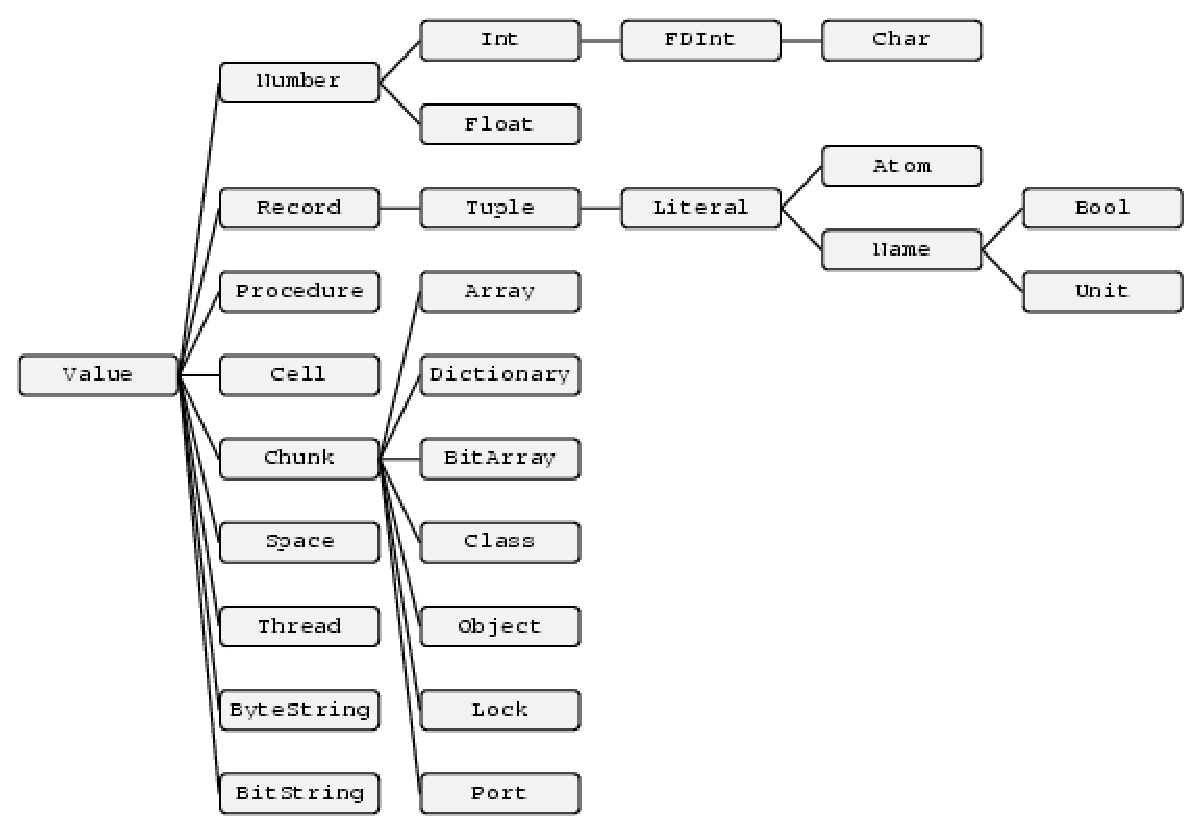
\includegraphics[width=0.70\textwidth]{../images/oz-datentypen} 
  \caption{Hierarchie der Datentypen in Oz 3. Quelle:
  \cite[Tutorial of Oz, Chapter 3.1]{url:mozart-documentation}}
  \label{fig:oz-datentypen}
\end{figure}

Einige der wichtigsten Datentypen seien hier kurz aufgeführt (vgl. 
\cite{Brunklaus:00}).

\begin{enumerate}
  \item Einfache Werte
    \begin{description}
      \item [Zahlen] können in Oz sowohl als ganze Zahlen (\texttt{Int, Char})
      als auch Fließkommazahlen (\texttt{Float}) benutzt werden.
      \item[Literale] teilen sich auf in sog. Atome und Namen. Ein Atom wird 
      durch eine alphanumerische Zeichenkette beschrieben, die entweder mit 
      einem Kleinbuchstaben beginnt oder in Hochkomma gefasst ist. Namen sind 
      eindeutige Bezeichner, die über eine spezielle Prozedur namens 
      \texttt{NewName} erzeugt werden können.
      \item[Prozeduren] können in Oz an Variablen gebunden und auch zur 
      Laufzeit erzeugt werden. \end{description}
  \item Zusammengesetzte Werte
    \begin{description}
      \item[Records] bestehen aus einem Bezeichner (Label) sowie einer festen 
      Anzahl von Komponenten oder Argumenten. Argumente bestehen aus dem Tupel 
      (Feature, Feld).
      \item[Tupel] sind ein Spezialfall von Records, bei denen die Argumente 
      kein explizites Feature besitzen.
      \item[Listen] sind eine Sonderform der Tupel. Die leere Liste wird mit
      \texttt{nil} denotiert, offene Listen bspw. als \texttt{1|2|3|nil} und 
      geschlossene Listen (also Listen mit fester Elementanzahl) als \texttt{[1 
      2 3]}.
    \end{description}
  \item \textbf{Chunks} erlauben es, abstrakte Datentypen zu konstruieren. 
  Oz bringt bereits einige vordefinierte Chunks mit, z.B. \texttt{Array} 
  oder \texttt{Dictionary}.
\end{enumerate}

\subsection{Multiparadigmisch?}
Wie bereits eingangs erwähnt, unterstützt Oz mehrere Programmierparadigmen:

\begin{enumerate}
  \item Constraint-Programmierung
  \item Funktionale Programmierung
  \item Objektorientierte Programmierung
  \item Logische Programmierung
\end{enumerate}
  
Im Gegensatz zu einer Programmiersprache, die nur eines der Paradigmen 
unterstützt, lassen sich in Oz also die zu lösenden Probleme von mehreren 
Seiten gleichzeitig mit dem jeweils geeignetsten Paradigma bearbeiten. 
Erreichen könnte man dies zwar auch durch die Kombination verschiedener 
Programmiersprachen, dabei bliebe aber der Nachteil, dass man semantische 
Lücken überwinden und Schnittstellen zwischen den einzelnen Sprachen definieren 
müsste. Dies würde u.a. zu einer aufwendigeren Fehlersuche führen. Mit Oz 
lassen sich hingegen die verschiedene Paradigmen problemlos miteinander 
kombinieren, deren gemeinsame Basis, das Oz Programming Model, im nächsten 
Abschnitt vorgestellt wird.

\subsection{Programmiermodell (Oz Programming Model, OPM)}
Die Grundlage für Berechnungen in Oz bildet das so genannte \textsl{Concurrent 
Constraint Programming}. Alle weiteren Paradigmen werden durch sog. "`syntactic 
sugar"' (Syntaxerweiterungen) in die Sprache integriert \cite{KI-LP96}.

Allgemein verwendet das Modell für Berechnungen die Metapher eines sog. 
\textsl{Berechnungsraums} (Computational Space). In diesem befindet sich zum 
einen ein \textsl{Speicher}, zum anderen eine Anzahl von sog. \textsl{Aktoren}. 
Aktoren führen die eigentlich Berechnung durch, indem sie schrittweise 
reduziert werden und sich dabei über den gemeinsamen Speicher synchronisieren. 
Dazu können Aktoren Information in den Speicher schreiben (tell) und auf 
Information warten und diese anfordern (ask).

Nebenläufigkeit (Concurrency) ist einer der wichtigsten Aspekte des OPM. Dabei 
bedeutet Nebenläufigkeit, dass verschiedene Berechnungen unabhängig voneinander 
durchgeführt werden können, nicht, dass diese parallel ablaufen.

\chapter{XML-�berblick}
\section{Was ist XML?} \label{xml-einfuehrung-was-ist}
Die erweiterbare Markup-Sprache \acr{xml} wurde im Jahre 1998 vom \acr{w3c} als Standard empfohlen und sollte den bereits seit den 80er Jahren existierenden Dokumentationsstandard \acr{sgml} vereinfachen und insbesondere f�r den Einsatz im Internet nutzbar machen.

\acr{xml} ist als echte Teilmenge von \acr{sgml} definiert -- sie wird daher auch als \acr{sgml}-Anwendungsprofil bezeichnet -- und bietet trotz starker Vereinfachungen eine gro�e M�chtigkeit bei der Definition neuer Dokumenten-Markups. \acr{xml} ist daher als \emph{Metasprache} -- also eine Sprache zur Definition anderer Sprachen -- zu bezeichnen, es handelt sich also weder um eine Programmiersprache noch ein Dateiformat.

Im Gegensatz zu \acr{html} (ebenfalls ein \acr{sgml}-Anwendungsprofil) ist das Markup bei \acr{xml} in seiner Semantik nicht statisch -- es k�nnen eigene Elemente definiert werden, die ihre Bedeutung erst bei Auswertung durch eine entsprechende Anwendung erhalten.

Zusammen mit den anderen um \acr{xml} entstandenen Architekturstandards (\zB \acr{xsd}, \acr{svg}, \acr{xslt}, oder XPath) bietet \acr{xml} heute eine breite und gut unterst�tzte Basis f�r webbasierte Technologien wie \acr{xhtml}, \acr{svg}, \acr{soap} oder auch \acr{rdf}.


\subsection{Geschichte}
Um die Entwicklung bis hin zum heutigen \acr{xml}-Standard aufzuzeigen, sind im folgenden einige der wichtigen chronologischen Eckdaten aufgef�hrt.

\begin{labeling}[~---]{\usekomafont{descriptionlabel}1980}%
	\item[\usekomafont{descriptionlabel}1980] 
		Erster Entwurf von \acr{sgml} durch die \acr{ansi} ver�ffentlicht
	\item[\usekomafont{descriptionlabel}1986] 
		\acr{iso} verabschiedet \acr{sgml} (\acr{iso} 8879:1986)
	\item[\usekomafont{descriptionlabel}1990] 
		Inbetriebnahme des "`World Wide Web"' -- erste einfache Versionen von \acr{html} und \acr{http}
	\item[\usekomafont{descriptionlabel}1992] 
		Erster Entwurf zu \acr{html}
	\item[\usekomafont{descriptionlabel}1994] 
		Gr�ndung des \acr{w3c}
	\item[\usekomafont{descriptionlabel}1996] 
		Erster Entwurf von \acr{xml} vorgestellt
	\item[\usekomafont{descriptionlabel}1998] 
		Erste Version von \acr{xml} durch das \acr{w3c} als "`Recommendation"' freigegeben
\end{labeling}

Im weiteren Verlauf wurden vom \acr{w3c} zahlreiche weitere Architekturstandards der \acr{xml}-Familie entwickelt und ver�ffentlicht.

\subsection{Entwurfsziele}
Die Entwickler -- die sog. \acr{xml} Working Group, eine Arbeitsgruppe unter der Schirmherrschaft des \acr{w3c} -- der \acr{xml}-Spezifikation \citep{url:W3C-XML-Spec} definierten die folgenden zehn Entwurfsziele \citep{url:W3C-XML-10P} f�r \acr{xml}:

\begin{enumerate}
	\item Einfache Nutzbarkeit �ber das/im Internet. \acr{sgml} als Ausgangspunkt wurde im Gegensatz dazu haups�chlich f�r den lokalen Einsatz (\zB f�r das Erstellen technischer Dokumentation) verwendet.
	\item Unterst�tzung eines breiten Anwendungsspektrums. Das oben bereits erw�hnte Haupteinsatzgebiet von SGML sollte durch \acr{xml} auf verschiedene Gebiete ausgeweitet werden.
	\item Kompatibilit�t zu \acr{sgml}. \acr{xml} ist als echte Untermenge des \acr{sgml}-Standards definiert, somit stellt jedes \acr{xml}-Dokument auch ein g�ltiges \acr{sgml}-Dokument dar und kann \zB �ber entsprechende Werkzeuge verarbeitet werden.
	\item Einfache Entwicklung \acr{xml}-verarbeitender Applikationen.
	\item Wenn m�glich, vollst�ndige Vermeidung optionaler Sprachelemente. Auf diese Weise soll die Komplexit�tsreduktion weiter gef�rdert werden, was wiederum der einfachen Benutzerbarkeit zugute kommt.
	\item \acr{xml}-Dokumente sollen menschenlesbar und hinreichend verst�ndlich sein.
	\item Z�giger Entwurf der \acr{xml}-Spezifikation. Dabei wurde der Umfang der \acr{sgml}-Spezifikation von ca. 600 auf 30 Textseiten deutlich reduziert.
	\item Formaler sowie pr�ziser Sprachentwurf. Dadurch sollte die schnelle und einfache Implementierung der \acr{xml}-Spezifikation in die entsprechenden Werkzeuge gew�hrleistet werden.
	\item Einfache Dokumentenerstellung. Im Normalfall soll f�r die Erstellung von \acr{xml}-Dokumenten kein spezielles Software-Werkzeug notwendig sein.
	\item Kompaktheit des Markups hat eine untergeordnete Priorit�t.
\end{enumerate}


\section{XML-Dokumente}
Im Sinne der \acr{xml}-Spezifikation wird ein Datenobjekt als \acr{xml}-\textbf{Dokument} bezeichnet, wenn es \emph{wohlgeformt} ist.

\subsection{Aufbau und Struktur}
Die Struktur eines \acr{xml}-Dokumentes l�sst sich in die Kategorien \emph{physisch} und \emph{logisch} aufteilen. Physisch gesehen besteht das Dokument aus einer Menge von Elementen. Ein Element kann dabei weitere Elemente enthalten; das Dokument beginnt mit dem sog. Dokument-Element.

Die logische Struktur eines Dokumentes besteht aus Elementen, Kommentaren, Deklarationen, Zeichenreferenzen und Verarbeitungsanweisungen. Es muss dabei darauf geachtet werden, dass die physischen und logischen Strukturen korrekt verschachtelt sind.

Ein \acr{xml}-Dokument besteht also aus den folgenden, teilweise optionalen Komponenten:

\begin{itemize}
	\item Prolog (optional): enth�lt \zB die verwendete \acr{xml}-Version (\zB \texttt{1.0}) sowie die Zeichenkodierung (\zB \texttt{UTF-8} oder \texttt{iso-8859-1})
	\item \acr{dtd}, Document Type Definition (optional): Verweis auf externe (bzw. direkte Angabe im Dokument) von Markup-Deklarationen
	\item Dokument-Element: Einzelnes Element, welches weitere Elemente enthalten darf.
	\item Kommentare an beliebiger Stelle au�erhalb des Markups
	\item Verarbeitungsanweisungen (PIs, Processing Instructions)
	\item \acr{cdata}-Abschnitte als Alternative zu Zeichendaten; Schutz ganzer Textbl�cke vor Interpretation als Markup
\end{itemize}

Der Grundbaustein eines Dokumentes ist also das \emph{Element}. Ein Element wird entweder durch Start- und End-Tags oder -- bei einem leeren Element -- durch ein Leeres-Element-Tag begrenzt. Weiterhin hat ein Element einen benannten Typ und kann eine Menge von Attributspezifikationen haben. Diese bestehen jeweils aus dem Komponenten \emph{Name} und \emph{Wert}. Abbildung \ref{fig:xml-strukturprimitive} veranschaulicht nochmals den Aufbau eines Elements.

\begin{figure}[htbp]
	\centering
		\includegraphics[width=0.70\textwidth,hiresbb=true]{images/xml-strukturprimitive}
	\caption{XML-Strukturkomponenten}
	\label{fig:xml-strukturprimitive}
\end{figure}

Aus logischer Sicht wird zwischen \textbf{analysierten} (parsed) und \textbf{nicht analysierten} (unparsed) Entities unterschieden. Analysierte Entities werden dabei �ber \emph{Entity-""Referenzen} angesprochen, nicht-analysierte direkt �ber ihren Namen.

\subsection{Wohlgeformtheit und Validit�t}
Ein \acr{xml}-Dokument wird als \textbf{wohlgeformt} bezeichnet, wenn es alle Wohlgeformtheitsbeschr�nkungen \citep{url:W3C-XML-Spec} einh�lt:

\begin{itemize}
	\item Der Name im End-Tag eines Elements muss mit dem Elementtyp im Start-Tag �bereinstimmen
	\item Attribute m�ssen eindeutig spezifiziert sein, d.h. kein Attribut darf mehrmalig im Start-Tag oder Leeres-Element-Tag vorkommen
	\item Elemente m�ssen sowohl Start- als auch End-Tag besitzen (ausgenommen leere Elemente: schlie�ender Schr�gstrich vor Tag-Ende)
	\item Attributwerte d�rfen keine direkten bzw. indirekten Referenzen auf externe Entities enthalten
	\item Attributwerte d�rfen das Zeichen \texttt{<} nicht enthalten
	\item Attributwerte m�ssen in Anf�hrungszeichen eingeschlossen sein
	\item Standalone-Dokumente ohne entsprechende \acr{dtd} m�ssen alle verwendeten Entities deklarieren (mit Ausnahme der vordefinierten)
\end{itemize}

Ein \acr{xml}-Dokument wird zudem als \textbf{valide} bezeichnet, wenn es die Eigenschaft erf�llt, eine Dokumenttyp-Deklaration zu besitzen und dieser zu entsprechen.

\section{Meta-Beschreibung von XML}
Um valide Dokumente erzeugen zu k�nnen, m�ssen die in einem Dokument zugelassenen Entity-Typen (samt deren Inhalten und zul�ssigen Attributen) definiert werden. Dazu gibt es die in den folgenden Abschnitten kurz beschriebenen Techniken.

\subsection{DTD -- Document Type Definition}
Eine \acr{dtd} ist eine schematische Beschreibung (mit eigenst�ndiger Syntax) eines \acr{xml}-Dokumentes und deklariert alle Elemente und Entities (definierte K�rzel wie \zB \texttt{\&amp;} in \acr{html}). Durch die Verkn�pfung eines Dokumentes mit einer \acr{dtd} kann erzwungen werden, dass sich das Dokument an eine gew�nschte Struktur h�lt (sog. \emph{Validierung}). 
Weiterhin lassen sich in einer \acr{dtd} Werte f�r Attribute oder Entities vorbelegen, sodass diese Werte zwischen verschiedenen Dokumenten geteilt und somit modular wiederverwendbar gemacht werden k�nnen.
Die konkrete Beschreibung des Aufbaus einer \acr{dtd} findet sich in der \acr{xml}-Spezifikation \citep{url:W3C-XML-Spec}.

\subsection{XSD -- XML Schema Definition} \label{einfuehrung-xml-xsd}
Als Nachfolger zu \acr{dtd} wurde \acr{xsd} als Schemasprache standardisiert. Gegen�ber \acr{dtd} bietet es u.a. folgende Vorteile (wobei bei \acr{xsd} alle Funktionalit�ten von \acr{dtd} eingeschlossen sind):

\begin{itemize}
	\item Syntax entspricht der eines \acr{xml}-Dokuments (kann also leicht validiert oder geparst werden)
	\item umfangreicher Vorrat an Datentypen
	\item Unterst�tzung f�r \acr{xml}-Namespaces
\end{itemize}

Ein Nachteil ist jedoch die relativ hohe Komplexit�t des \acr{xsd}-Konzeptes.

\section{Beispieldokument}
Ein wohlgeformtes, valides \acr{xml}-Beispieldokument zeigt Listing \ref{listing:xml-beispiel}. Die \acr{dtd} wird dabei nicht extern referenziert sondern ist direkt im oberen Teil des Dokumentes enthalten.

\lstinputlisting[language=XML,caption={XML-Beispieldokument},label=listing:xml-beispiel]{Kapitel/Einfuehrung/beispiel.xml}

\section{Verarbeitung von XML-Dokumenten}
Um ein \acr{xml}-Dokument zu verarbeiten, muss zun�chst eine Analyse der Dokumentenstruktur (\emph{Parsing}) vorgenommen werden. Die zwei Standardans�tze dazu sind in den nachfolgenden Unterabschnitten beschrieben.

\subsection{DOM -- Document Object Model} \label{xml-einfuehrung-dom}
Bei dem Document Object Model handelt es sich um eine vom \acr{w3c} standardisierte \citep{url:W3C-DOM-Core}, plattform- und sprachunabh�ngige Zugriffsmethode f�r \acr{xml}-Dokumente. Eine ganze Reihe von Empfehlungen definieren dabei u.a. Funktionen zur Navigation innerhalb von \acr{xml}-Dokumenten oder deren Manipulation.

Das \acr{dom} basiert auf einem \textbf{Baummodell} des Dokumentes -- dabei gibt es verschiedene Knotentypen, die \zB das Dokument-Element, andere Elemente oder Attribute darstellen. Auf diese Knoten k�nnen dann verschiedene Operationen durchgef�hrt werden; so lassen sich \zB alle Kindknoten, der Elternknoten oder der Wert eines Attributes ermitteln.

Das Beispieldokument aus Listing \ref{listing:xml-beispiel} lie�e sich \zB durch den Baum in Abbildung \ref{fig:xml-beispiel-baumdarstellung} darstellen.
\begin{figure}
	\centering
		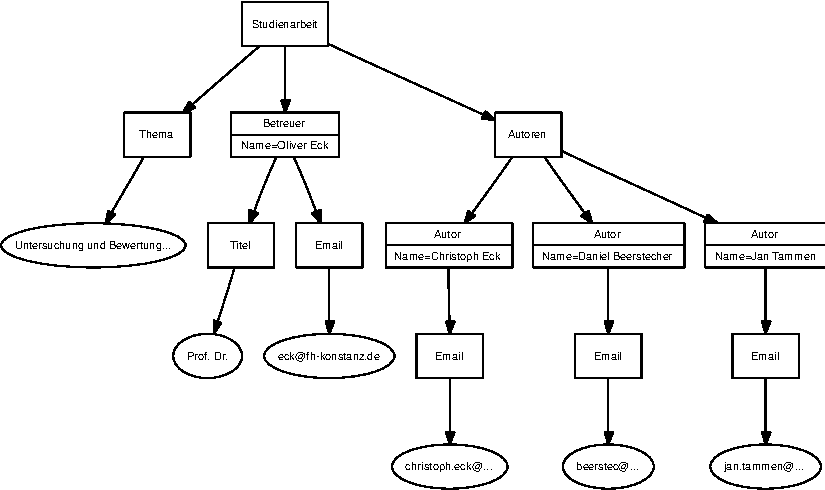
\includegraphics[width=1.00\textwidth]{images/xml-beispiel-baumdarstellung}
	\caption{Baumdarstellung des Beispiel-Dokumentes}
	\label{fig:xml-beispiel-baumdarstellung}
\end{figure}


\subsection{SAX -- Simple API for XML} \label{xml-einfuehrung-sax}
Im Gegensatz zur baumbasierten Verarbeitung beim \acr{dom} wird mit \acr{sax} \emph{ereignisorientiert} auf ein \acr{xml}-Dokument zugegriffen. Das bedeutet, dass beim Auftreten bestimmter Analysergebnisse (\zB Beginn oder Ende eines Elements) Ereignisse ausgel�st werden. Somit kann \zB �ber einen Callback-Mechanismus je nach Ereignis eine geeignete Methode aufgerufen werden, welche die Daten dann entsprechend verarbeiten muss.

Ein Vorteil dieses Ansatzes ist die sequentielle Verarbeitung der Daten, wodurch nicht das komplette Dokument im Speicher gehalten werden muss. Zum Nachteil wird diese Tatsache jedoch dann, wenn zur Verarbeitung viele �ber das Dokument verstreute Informationen ben�tigt werden und somit die Anzahl der Zugriffe stark ansteigt.

Die Verarbeitung des Beispieldokumentes w�rde nacheinander die folgenden \acr{sax}-Ereignisse (vereinfachte Darstellung: es wird u.a. die DTD ignoriert) erzeugen:

\begin{enumerate}
	\item \texttt{startDocument}
	\item \texttt{startElement}("`Studienarbeit"')
	\item \texttt{startElement}("`Thema"')
	\item \texttt{characters}("`Untersuchung und Bewertung..."')
	\item \texttt{startElement}("`Betreuer"', AttributeList(length = 1, {name = 'Name', type = 'PCDATA', value = 'Oliver Eck'}))
	\item \texttt{startElement}("`Titel"')
	\item \texttt{characters}("`Prof. Dr."')
	\item \texttt{endElement}("`Titel"')
	\item \texttt{startElement}("`Email"')
	\item \texttt{characters}("`eck@fh-konstanz.de"')
	\item \texttt{endElement}("`Email"')
	\item \texttt{endElement}("`Betreuer"')
	\item \ldots
	\item \texttt{endDocument}
\end{enumerate}

\section{Anwendungsf�lle f�r den XML-Einsatz}
\begin{itemize}
	\item Datentransfer innerhalb einer Applikation
	\item Integration von bestehenden Applikationen in neue Systeme
	\item E-Commerce, B2B (\zB bietet das Internetversandhaus Amazon.com einige seiner Dienste �ber WebServices an \citep{url:amazon})
	\item Content-Management und -Publishing
	\item Datenspeicherung, \zB Konfigurationsdaten oder auch als Dateiformat (s. OpenDocument)
	\item Datenspeicherung in Datenbanken, \zB Bestelldaten, Reservierungen
\end{itemize}

\section{St�rken von XML}
Laut \citep[Kap. 22]{Ambler2003} und \citep[Kap. 3]{Schoening2003} sind es vor allem die folgenden Punkte, welche f�r den Einsatz von \acr{xml} sprechen.

\begin{itemize}
	\item \acr{xml} ist plattform- sowie programmiersprachenunabh�ngig und kann somit auf den unterschiedlichsten Computersystemen gelesen und geschrieben werden
	\item Beim Einsatz von \acr{xml} entstehen keine Lizenzkosten. Die \acr{xml}-""Spezifikation wird kostenlos vom \acr{w3c} �ber das Internet zur Verf�gung gestellt und kann auch in kommerziellen Produkten weiterverwendet werden.
	\item Weiterhin existiert eine gro�e Anzahl von (kostenlosen oder gar quelloffenen) Werkzeugen f�r die Arbeit mit \acr{xml}, wie \zB Editoren, Parser oder Datenbanken.
	\item Ein gro�er Vorteil f�r die Internationalisierung von Software ist die Tatsache, dass \acr{xml} auf Unicode basiert.
	\item Die Familie der \acr{xml}-Technologien ist (weitgehend) standardisiert und wird laufend aktualisiert und erweitert.
	\item \acr{xml} ist in der Industrie bereits weit verbreitet und akzeptiert
	\item \acr{xml}-Dokumente \emph{k�nnen} von Menschen gelesen werden -- dies ist vor allem bei Fehlersuchen o.�. Szenarien von Vorteil.
	\item �ber \zB \acr{xsl} k�nnen Inhalt und Darstellung von \acr{xml}-Dokumenten leicht getrennt werden. Dies entspricht dem allgemeinen Trend zur Separation von Struktur und Darstellung (s. "`semantisches Web"').
%	\item Bei sehr komplex strukturierten Gesch�ftsdaten bedeutet der Einsatz \acr{xml} oftmals eine Verk�rzung der Entwicklungszeit.
\end{itemize}


\section{Schw�chen von XML}
Offensichtlich gibt es auch einige Nachteile beim Einsatz von \acr{xml} -- \citep[Kap. 22]{Ambler2003} erw�hnt dazu die folgenden Themen:

\begin{itemize}
	\item \acr{xml}-Dokumente neigen dazu, sehr ausf�hrlich zu werden (\zB durch die Benutzung langer Elementnamen. Dies wirkt sich negativ auf den Speicherbedarf aus. Bei dem heutigen Entwicklungsstand der Speichermedien (hohe Kapazit�t zu geringen Preisen) ist dieser Punkt jedoch vernachl�ssigbar und wird durch den Vorteil, dass Dokumente durch die gr��ere Ausf�hrlichkeit auch leichter verst�ndlich werden, noch weniger bedeutsam.
	\item \acr{xml}-Dokumente m�ssen st�ndig, um \zB in einer Software-""Applikation in ein Objekt �berf�hrt oder in einer Datenbank gespeichert werden zu k�nnen, geparst werden. Andere Speicherformen k�nnen somit u.U. performanter sein.
	\item Einige der \acr{xml}-Standards sind z.Z. noch in der Entwicklung und man kann sich nicht darauf verlassen, dass diese Standards �berhaupt allgemeing�ltig akzeptiert werden. Dies ist jedoch stets eine Gefahr im Zusammenhang mit Standards und somit kein \acr{xml}-spezifisches Problem.
\end{itemize}


\section{Die XML-Sprachfamilie}
In Tabelle \ref{tab:xml-standards} sind einige der zur \acr{xml}-Familie geh�renden Sprachen und Standards aufgef�hrt.
\begin{table}
	\sffamily
	\centering
	%\footnotesize
	\begin{tabularx}{\textwidth}{lX}
		\toprule
		
		\multicolumn{1}{@{}N}{Bezeichnung} & \multicolumn{1}{V{6em}@{}}{Beschreibung} \\
		%\cmidrule(r){1-1}\cmidrule(l){2-2}		
		\midrule\addlinespace\addlinespace
		
		\acr{xsl} 			& Sprachfamilie zur Layout-Erzeugung f�r \acr{xml}-Dokumente. Zu \acr{xsl} geh�ren \acr{xslt} und \acr{xsl-fo} \\ \cmidrule{1-2}
		\acr{xslt} 			& Geh�rt zur \acr{xsl}-Familie und dient zur Transformation von Dokumenten in andere Formate. �ber \acr{xslt}-Stylesheets l�sst sich \zB ein \acr{xml}-Dokument in ein \acr{html}- bzw. \acr{xhtml}-Dokument transferieren, um es �ber einen Webbrowser anzuzeigen.\\ \cmidrule{1-2}
		XLink 					& Syntax zur Definition von bi- oder auch multidirektionalen, externen Links in \acr{xml}.\\ \cmidrule{1-2}
		XPointer 				& Auch "`\acr{xml} Pointer Language"'. Anfragesprache, um mittels XLink-Ausdr�cken bzw. in URIs auf einzelne Teile eines \acr{xml}-Dokumentes zu verweisen.\\ \cmidrule{1-2}
		XML Namespaces 	& �ber Namensr�ume soll die Eindeutigkeit von \acr{xml}-Elementen sichergestellt und somit Namenskollisionen verhindert werden. \\ \cmidrule{1-2}
		XML Signature 	& Schreibweise f�r das Signieren von \acr{xml}-Dokumenten. \\ \cmidrule{1-2}
		XML-Encryption 	& Spezifikation f�r das Ver- und Entschl�sseln von \acr{xml}-""Dokumenten. \\ \cmidrule{1-2}
		\acr{xsd} 			& Siehe Kapitel \ref{einfuehrung-xml-xsd}. \\ \cmidrule{1-2}
		\acr{xhtml} 		& Auf \acr{xml} basierender Nachfolger von \acr{html}. \\ \cmidrule{1-2}
		\acr{svg} 			& Erm�glicht die Beschreibung von 2D--Vektor Grafiken in \acr{xml}. \\ \cmidrule{1-2}
		\acr{soap} 			& �ber dieses Protokoll k�nnen Daten zwischen Systemen ausgetauscht, sowie \acr{rpc}s durchgef�hrt werden. \\ \cmidrule{1-2}
		\acr{rdf} 			& Dient zur Repr�sentation von Metadaten. \\ \cmidrule{1-2}
		XPath 					& Siehe Kapitel \ref{einfuehrung-xml-xpath}. \\ \cmidrule{1-2}
		XQuery 					& Siehe Kapitel \ref{einfuehrung-xml-xquery}. \\
								
		\addlinespace
		\bottomrule
		
		\end{tabularx}
	\caption{Einige XML-Architekturstandards}
	\label{tab:xml-standards}
\end{table}

Im Zusammenhang mit Datenbanken sind \emph{XPath} sowie \emph{XQuery} von besonderer Bedeutung, deshalb wird auf diese Standards in den folgenden Abschnitten n�her eingegangen.

\subsection{XPath} \label{einfuehrung-xml-xpath}
Mit XPath lassen sich die Elemente eines \acr{xml}-Dokuments adressieren. XPath ist keine eigenst�ndige Sprache. Vielmehr bauen andere Sprachen wie etwa \acr{xslt} oder XQuery darauf auf. 

XPath wurde vom \acr{w3c} in der Version 1.0 standardisiert. Es existiert bereits eine Empfehlung f�r XPath 2.0, die mindestens bis zum 28. Januar 2006 bestehen bleiben soll. Anschlie�end soll XPath 2.0 verabschiedet werden \citep{url:heise-online}.

Bei XPath wird jedes \acr{xml}-Dokument als Baum angesehen \citep{url:obqo}. Mit XPath kann jeder Knoten dieses Baumes angesprochen werden. Jeder sogenannte Lokalisierungspfad besteht aus drei Teilen:
\begin{itemize}
	\item Einer Achse
	\item Einem Knotentest
	\item Einem Pr�dikat
\end{itemize}

In XPath werden eine Reihe von verschiedenen Knotentypen unterschieden:
\begin{itemize}
	\item Wurzelknoten (root node)
	\item Elementknoten (element node)
	\item Kommentarknoten (command node)
	\item Textknoten (text node)
	\item Namensraumknoten (namespace node)
	\item Verarbeitungsanweisungsknoten (processing instruction node)
\end{itemize}

Jeder Knoten kann �ber einen Lokalisierungspfad angesprochen werden. Der Lokalisierungspfad ist immer relativ zu dem momentanen Knoten. Dieser momentane Knoten wird als Kontextknoten bezeichnet.

Im Folgenden einige Beispiele f�r Lokalisierungspfade:
\begin{itemize}
	\item \texttt{child::b} - w�hlt den Knoten \texttt{b} des Kontextknotens aus.
	\item \texttt{child::*} - w�hlt alle Knoten des Kontextknotens aus.
	\item \texttt{attribut:c} - w�hlt das Attribut \texttt{c} des Kontextknotens aus.
	\item \texttt{/} - w�hlt die Wurzel des Dokuments aus.
\end{itemize}

\subsubsection{Achsen}
Als Achsen wird in XPath eine bestimmte Gruppe von Knoten bezeichnet. Es werden die folgenden Achsen unterschieden:
\begin{itemize}
	\item Child (Kind): Alle Knoten, die unmittelbar unter dem Kontextknoten liegen
  \item Descendant (Nachkomme): Alle dem Kontextknoten nachfolgenden Knoten. Im Gegensatz zum Child umfasst der Descendant nicht nur die Knoten der n�chsten Ebene, sondern alle unter dem Kontextknoten liegenden Knoten.
	\item Parent (Eltern): Der Knoten, der dem Kontextknoten unmittelbar �bergeordnet ist. Der Wurzelknoten besitzt als einziger aller Knoten keinen Parent.
	\item Ancestor (Vorfahre): Ancestor sind alle Elternknoten des Kontextknoten, also den Elternknoten des Kontextknotens sowie den Elternknoten des Elternknotens und wiederum dessen Elternknoten usw.
	\item Following-sibling (Nachfolgende Geschwisterknoten): Alle nachfolgenden Knoten, die nach dem Kontextkonten im Dokument auftreten, jedoch ohne At"-tri"-but- und Namensraumknoten und ohne die Nachkommen.
	\item Preceding-sibling (Vorherige Geschwisterknoten): Alle vorherigen Geschwisterknoten des Kontextknotens.
	\item Following (nachfolgende Knoten): Alle nachfolgenden Knoten, die nach dem Kontextkonten im Dokument auftreten, jedoch ohne Attribut- und Namensraumknoten.
	\item Preceding (vorherige Knoten): Alle vorherigen Knoten, dir vor dem Kontextkonten im Dokument auftreten, jedoch ohne Vorfahren, Attribut- und Namensraumknoten.
	\item Attribute (Attribut): Attributknoten
	\item Namespace (Namensraum): Namensraumknoten
	\item Self (aktueller Knoten): Ist der Kontextknoten selbst.
	\item Descendant-or-self (Nachkomme und aktueller Knoten): Erh�lt alle Nachkommen sowie den Kontextknoten.
	\item Ancestor-or-self (Vorfahre und aktueller Knoten): Erh�lt die Vorfahren des Kontextknoten sowie den Kontextknoten selbst. 
\end{itemize}

\begin{figure}[htbp]
	\centering
		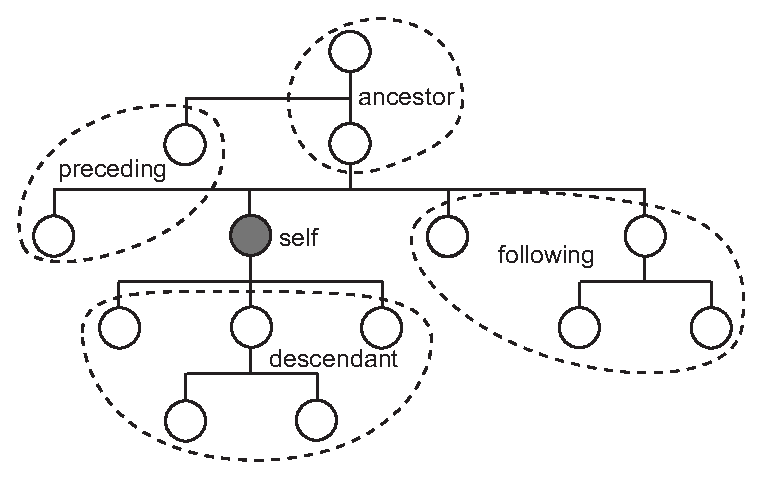
\includegraphics{images/baum_xpath.eps}
	\caption{XPath Baumstruktur}
	\label{fig:baum_xpath}
\end{figure}


\subsubsection{Knotentests}
Achsen besitzen sogenannte Hauptknotentypen. Eine Achse, die aus Elementen besteht, hat als Hauptknotentyp den Elementtyp; eine Achse, die aus Attributen besteht, hat als Hauptknotentyp den Attributtyp usw.

Beim Knotentest werden diejenigen Knoten untersucht, die vom Typ Knotentest sind. Mit dem Knotentest werden die Knoten, die �ber die Achsen ausgew�hlt wurden, noch weiter eingeschr�nkt. Es gibt die folgenden Knotentests:

\begin{itemize}
	\item \texttt{*} - Der Knotentest ist f�r jede Bedingung des Hauptknotentyps erf�llt.
	\item \texttt{text()} - Der Knotentest ist f�r jeden Textknoten erf�llt.
	\item \texttt{comment()} - Der Knotentest ist f�r jeden Kommentarknoten erf�llt.
	\item \texttt{processing-instruction()} - Der Knotentest ist f�r jede Processing Instruction g�ltig.
	\item \texttt{node()} - Der Knotentest ist f�r jeden Knoten g�ltig.
\end{itemize}

\paragraph{Beispiele}
\begin{itemize}
	\item \texttt{child::*} - w�hlt alle Kindknoten des Hauptknotentyps bezogen auf den Kontextknoten aus 
	\item \texttt{child::text()} - w�hlt alle Kindknoten des Typs \texttt{text} bezogen auf den Kontextknoten aus
\end{itemize}

\subsubsection{Pr�dikate}

Bei Pr�dikaten handelt es sich um eine weitere Einschr�nkung der Knoten. Die Pr�dikate werden in eckige Klammern geschrieben.

\paragraph{Beispiele}
\begin{itemize}
	\item \texttt{//Studienarbeit/Autoren/Autor[@Name = ''Jan Tammen'']}: W�hlt denjenigen Knoten aus, bei dem das Attribut \texttt{Name} den entsprechenden Wert besitzt: \texttt{<Autor Name=''Jan Tammen''>...</Autor>}.
	\item \texttt{//Studienarbeit/Autoren/Autor[1]}: W�hlt das erste Element vom Typ \texttt{Autor} im Dokument aus: \texttt{<Autor Name=''Christoph Eck''>...</Autor>}.
\end{itemize}

\subsubsection{Kurzschreibweisen}
Tabelle \ref{tab:Kurzschreibweisen} zeigt h�ufig verwendete Kurzschreibweisen in XPath (nach \citep{url:tu-chemniz}).
\begin{table}
	\sffamily
	\centering
	
	\begin{tabularx}{\textwidth}{llX}
		\toprule
		
		\multicolumn{1}{@{}N}{Zeichen} & \multicolumn{1}{V{6em}@{}}{Abk�rzung f�r} & \multicolumn{1}{V{6em}@{}}{Bedeutung} \\
		\midrule\addlinespace\addlinespace
		
		\texttt{//}	& \texttt{/descendant-or-self::node()/} 	& Alle Nachkommen und Kontextknoten \\  %\cmidrule{1-3}
		\texttt{.}	& \texttt{self::node()} 									& Der Kontextknoten \\  %\cmidrule{1-3}
		\texttt{..}	& \texttt{parent::node()} 								& Eltern des Kontextknoten \\  %\cmidrule{1-3}
		\texttt{@} 	& \texttt{attribute::} 										& Attribut ausw�hlen	\\
		
		\addlinespace
		\bottomrule
		\end{tabularx}
	\caption{Kurzschreibweisen}
	\label{tab:Kurzschreibweisen}
\end{table}

\subsection{XQuery} \label{einfuehrung-xml-xquery}
XQuery ist ein Abfragesprache, die vom \acr{w3c} entworfen wurde. Mindestens bis zum 28. Februar 2006 soll XQuery als Empfehlung stehen bleiben, anschlie�end soll der Standard verabschiedet werden \citep{url:heise-online}.

XQuery basiert auf XPath, das hei�t, es verwendet f�r die Bezeichnung der Elemente innerhalb des \acr{xml}-Dokumentes XPath.

\subsubsection{FLWOR-Ausdr�cke}
Umfangreichere XQuery-Abfragen arbeiten mit sogenannten FLWOR-Ausdr�cken. FLWOR (ausgesprochen 'flower') steht f�r "`For-Let-Where-Order by-Return"':

\begin{itemize}
	\item \texttt{for}: Bindet eine Liste von Werte an Variablen.
	\item \texttt{let}: Bindet einen einzelnen Wert an eine Variable.
	\item \texttt{where}: Nach \texttt{where} - erfolgt ein Ausdruck, der \texttt{true} oder \texttt{false} sein kann.
	\item \texttt{order by}: Sortiert die Liste aufsteigend (Voreinstellung) oder absteigend.
	\item \texttt{return}: Definiert den R�ckgabewert des Ausdruckes. Die Klausel wird f�r jedes Tupel des Ergebnisstroms einmal evaluiert.
\end{itemize}

\paragraph{Beispiel}
Das folgende Beispiel eines FLWOR-Ausdruckes benutzt einige der in XQuery integrierten Funktionen und ermittelt diejenigen Studenten, bei denen der Nachname mit einem "`B"' beginnt.

\lstinputlisting[language=XQuery,caption={XQuery Beispielabfrage},label=listing:xquery-flwor-beispiel]{Kapitel/Einfuehrung/beispiel.xql}

Das konstruierte Ergebnis sieht wie folgt aus:
\lstinputlisting[language=SQL,caption={Ergebnis der XQuery Beispielabfrage},label=listing:xquery-flwor-beispiel-ergebnis,language=XML]{Kapitel/Einfuehrung/beispiel-ergebnis.xql.xml}

Joins lassen sich erstellen, indem zwei Listen von Werten mit \texttt{for} gebunden werden.
Neben dem FLWOR-Audruck beherrscht XQuery eine \texttt{if-then-else} Konstruktion:

\lstinputlisting[language=XQuery,caption={If-then-else Konstruktion in XQuery},label=listing:xquery-if-then-else]{Kapitel/Einfuehrung/if-then-else.xql}

Wenn \texttt{expr1} wahr ist, wird \texttt{expr2} zur�ckgeliefert, ist \texttt{expr1} falsch, so wird \texttt{expr3} zur�ckgeliefert.

\subsubsection{Funktionen}
XQuery besitzt �ber 100 vordefinierte Funktionen. Tabelle \ref{tab:xquery-funktionen} zeigt einige Beispiele f�r solche Funktionen -- dabei wird auf die Angabe der exakten Funktions-Signaturen verzichtet.

\begin{table}
	\sffamily
	\centering
	\begin{tabularx}{\textwidth}{lX}
		\toprule
		
		\multicolumn{1}{@{}N}{Funktionsbezeichnung} & \multicolumn{1}{V{6em}@{}}{Beschreibung} \\
		\midrule\addlinespace\addlinespace

		\texttt{string-join()}	& Verbindet zwei Zeichenketten miteinander. \\ \cmidrule{1-2}
		\texttt{compare()} 			& Vergleicht zwei Zeichenketten. \\ \cmidrule{1-2}
		\texttt{substring()} 		& Pr�ft, ob die Zeichenkette in einer zweiten Zeichenkette erhalten ist. \\ \cmidrule{1-2}
		\texttt{document()}			& Datei �ffnen \\ \cmidrule{1-2}
		\texttt{tokenize()}			& Trennt den �bergabestring anhand eines regul�ren Ausdrucks in mehrere Teile auf. \\ \cmidrule{1-2}
		\texttt{starts-with()}	& Pr�ft, ob ein �bergebener String mit einer bestimmten Zeichenkette beginnt. \\
		
		\addlinespace
		\bottomrule
		\end{tabularx}
	\caption{Einige XQuery-Funktionen}
	\label{tab:xquery-funktionen}
\end{table}


\subsection{XSLT}
Mithilfe der \acr{xslt}-Programmiersprache, die Teil von \acr{xsl} ist, k�nnen \acr{xml}-""Dokumente in beliebige Strukturen (\zB \acr{xhtml}, \acr{wml}, VoiceXML, \ldots) transformiert werden. Dazu werden einem \acr{xslt}-""Prozessor �ber \acr{xslt}-""Dokumente, sog. "`Stylesheets"' (bzw. richtiger "`Transformationssheets"', s. \citep{Herpers2002}), mitgeteilt, wie die einzelnen \acr{xml}-Elemente transformiert werden sollen.
�hnlich wie beim \acr{dom} wird das Dokument als Baum interpretiert; �ber XPath (s. \ref{einfuehrung-xml-xpath}) k�nnen die einzelnen Baum-Elemente angesprochen bzw. selektiert werden.

\subsubsection{Beispieldokument}
In Listing \ref{listing:xslt-beispiel} ist ein Beispiel f�r ein \acr{xslt}-Transformationssheet aufgef�hrt. Es dient dazu, das \acr{xml}-Dokument aus Listing \ref{listing:xml-beispiel} in ein \acr{xhtml}-Dokument zu transformieren, sodass es �ber einen Webbrowser angezeigt werden kann. Anhand dieses Beispiels wird dann der allgemeine Aufbau eines \acr{xslt}-Dokuments beschrieben.

\lstinputlisting[language=XSLT,caption={XSLT-Beispieldokument},label=listing:xslt-beispiel]{Kapitel/Einfuehrung/beispiel.xsl}

\subsubsection{Aufbau eines XSLT-Dokuments}
Da es sich bei einem \acr{xslt}-Dokument um eine \acr{xml}-Anwendung handelt, beginnt das Dokument zun�chst mit der entpsrechenden \acr{xml}-Deklaration. Anschlie�end folgt das eigentliche "`Stylesheet"' im Element \texttt{<xsl:transform>}.
Hauptbestandteil eines \acr{xslt}-Dokuments sind die sog. Transformationsregeln (Template Rules), die wie folgt aufgebaut sind: 

\begin{lstlisting}[language=XSLT,numbers=none]
<xsl:template match="/ein/XPath/Ausdruck"> [...] </xsl:template>
\end{lstlisting}

�ber das Attribut \texttt{match} wird mithilfe eines XPath-Ausdruckes bestimmt, f�r welchen Knoten diese Regel gilt. Innerhalb des Elements wird dann \zB das auszugebende Markup sowie weitere Anweisungen eingetragen.

Mittels der Anweisung \texttt{<xsl:attribute name=.../>} kann ein Attribut f�r das aktuelle Element hinzugef�gt werden, in unserem Beispiel das \texttt{href}-Attribut des \texttt{<a>}-Elements.

Die Anweisung \texttt{<xsl:apply-templates select=.../>} veranlasst den \acr{xslt}-""Prozessor dazu, entsprechende Templates f�r alle Kindknoten des aktuellen Knotens zu suchen und anzuwenden. �ber die optionale Angabe des Attributs \texttt{select} kann ein spezielles Template angesteuert werden.

Weitere Sprachelemente wie Bedingungen (\texttt{<xsl:if>, <xsl:choose>}), Sortierungen (\texttt{<xsl:sort>}) oder Schleifen (\texttt{<xsl:for-each>}) sind in unserem einfachen Beispiel nicht enthalten; deren Funktionsweise kann bei Bedarf \zB in der \acr{xslt}-Spezifikation \citep{url:Clark1999} nachgelesen werden.

Nach Anwendung des \acr{xslt}-""Transformationssheets auf unser Quell-Dokument (entweder serverseitig durch einen externen oder einen in den Webbrowser integrierten \acr{xslt}-Prozessor) ergibt sich der folgende \acr{xhtml}-Code:

\lstinputlisting[language=HTML,caption={Ergebnis der Transformation},label=listing:xslt-ergebnis]{Kapitel/Einfuehrung/beispiel.xhtml}

\section{�nderungsoperationen auf XML-Dokumente}
Im Gegensatz zu \acr{sql} -- mit seinen \acr{dml}-Befehlen \texttt{INSERT}, \texttt{DELETE} und \texttt{UPDATE} -- bietet XQuery im derzeitigen Stadium \emph{keine} M�glichkeit, �nderungsoperationen an Dokumenten durchzuf�hren \citep{url:Champion2004, url:Klettke2005}.
Da aber \zB das Einf�gen bzw. Ab�ndern einzelner Elemente oder Attribute eines \acr{xml}-Dokumentes durchaus w�nschenswerte Funktionen sind, haben sich eine Reihe von entsprechenden Erweiterungen verbreitet. 

\subsection{XUpdate}
Eine dieser Erweiterungen -- genannt "`XUpdate"' -- wurde von der \acr{xml}:DB-Initiative\footnote{\url{http://xmldb-org.sourceforge.net/}} vorgeschlagen und liegt derzeit als "`Working Draft"' aus dem Jahre 2000 vor \citep{url:Laux2000}. Einige der wichtigsten f�r XUpdate definierten Anwendungsf�lle \citep{url:Staken} sind:

\begin{itemize}
	\item Einf�gen eines neuen Elements vor/nach einem Element
	\item Einf�gen eines Attributs
	\item Text-Inhalt in ein Element einf�gen
	\item Element/Attribut aktualisieren
	\item Element/Attribut umbenennen, l�schen
	\item usw.
\end{itemize}

Die XUpdate-Syntax wird z.Z. von einigen nativen \acr{xml}-\acr{dbms} wie \zB dbXML oder eXist unterst�tzt.

\subsection{XQuery-Erweiterungen}
Die XQuery-Spezifikation wurde so entwickelt, dass die geforderten Update-""Funktionen prinzipiell sp�ter noch erg�nzt werden k�nnen. Es liegt ein entsprechender Working Draft \citep{url:Chamberlin2005} vor, welcher �hnliche Anwendungsf�lle f�r eine m�gliche XQuery-Erweiterung wie bei XUpdate definiert, diese aber etwas allgemeiner formuliert:

\begin{itemize}
	\item Aktualisierung von \acr{xml}-Dokumenten in persistenten Speichermedien
	\item Hinzuf�gen neuer Daten zu \acr{xml}-Dokumenten
	\item Erzeugen editierter Dokumenten-Kopien
	\item Transaktionssicherheit (\acr{acid}-Prinzip)
\end{itemize}

Da nicht damit gerechnet wird, dass entsprechende Erweiterungen in der n�chsten Zeit in die XQuery-Spezifikation einflie�en werden, haben sich diverse Vorschl�ge entwickelt, die teilweise auf der Arbeit von \citep{Lehti2001} aufbauen.

\chapter{ISO/ANSI-Standard: SQL/XML}
Mit der Revision des \acr{sql}-Standards 2003 wurde \acr{sql} unter anderem um \acr{xml}-F�higkeiten erweitert. Diese Erweiterung wird h�ufig auch als \acr{sql}/\acr{xml} bezeichnet. Im Gegensatz zu z.B. XPath wurde \acr{sql}/\acr{xml} \emph{nicht} vom \acr{w3c} standardisiert, sondern von der ISO/ANSI. 

Die Erweiterungen des Standards erlaubt es, \acr{xml}-Daten in einer relationalen Datenbank abzulegen oder aus Daten \acr{xml}-Dokumente zu generieren. 

\section{Der Datentyp XML}
Mit \acr{sql}/\acr{xml} wurde der neue Datentyp \texttt{XML} eingef�hrt, der in der Lage ist, \acr{xml}-Daten aufzunehmen \citep{Tuerker2003}.  Das folgende Beispiel zeigt eine Tabelle "`Lieferant"', die ein Feld "`Bemerkungen"' besitzt, in dem \acr{xml}-Daten eingef�gt werden k�nnen:

\lstinputlisting[language=SQL,caption={Create Table mit Datentyp XML},label=listing:xml-create-table,morekeywords={XML}]{Kapitel/Einfuehrung/CreateTable.txt}

Der Datentyp \texttt{XML} erlaubt die Speicherung folgender Daten:
\begin{itemize}
	\item \texttt{NULL}
	\item \acr{xml}-Inhalte
	\item \acr{xml}-Dokumente (\acr{xml}-Daten mit Vorspann)
\end{itemize}

\section{XML-Funktionen} \label{einf�hrung-sqlxml-funktionen}
\acr{sql} wurde um die folgenden \acr{xml}-Funktionalit�ten erweitert:
\begin{itemize}
	\item \texttt{XMLGEN}: Erm�glicht das Einf�gen von XQuery-Abfragen.
	\item \texttt{XMLELEMENT}: Erzeugt ein \acr{xml}-Element
	\item \texttt{XMLATTRIBUTES}: Erzeugt ein \acr{xml}-Attribut
	\item \texttt{XMLFOREST}: Erzeugt einen Wald von \acr{xml}-Elementen
	\item \texttt{XMLCONCAT}: konkateniert \acr{xml}-Elemente
	\item \texttt{XMLAGG}: Funktion zum Aggregieren oder gruppieren von \acr{xml}-Werten. 
\end{itemize}

Hinweis: Alle \texttt{XML}-Funktionen -- au�er XMLAGG -- k�nnen �ber \texttt{XMLGEN} und XQuery nachgebildet werden.

\section{Abbildung zwischen SQL und XML}
\acr{sql} und \acr{xml} basieren auf unterschiedlichen Datenmodellen. Daher muss das \acr{sql}-Datenmodell auf das \acr{xml}-Datenmodell abgebildet werden und umgekehrt. Diese Abbildung zeigt Tabelle \ref{tab:abbildung-sql-xml}.

\begin{table}
	\sffamily
	\centering
	
	\begin{tabularx}{\textwidth}{lX}
		\toprule
		
		\multicolumn{1}{@{}N}{\acr{sql}-Datenmodell} & 	 \multicolumn{1}{V{6em}@{}}{\acr{xml}-Datenmodell} \\
		\midrule\addlinespace\addlinespace

		\acr{sql}-Bezeichner 		& \acr{xml}-Name \\ %\cmidrule{1-2}
		\acr{sql}-Zeichens�tze 	& \acr{xml}-Unicode \\ %\cmidrule{1-2}
		\acr{sql}-Datentypen 		& \acr{xml}-Schema-Typen \\ %\cmidrule{1-2}
		\acr{sql}-Tabelle 			& \acr{xml}-Dokument \\ %\cmidrule{1-2}
		\acr{sql}-Schemata 			& \acr{xml}-Dokument + \acr{xml}-Schema-Dokument \\ %\cmidrule{1-2}
		\acr{sql}-Katalog 			& \acr{xml}-Dokument + \acr{xml}-Schema-Dokument \\ 
		\addlinespace
		\bottomrule
		\end{tabularx}
	\caption{Abbildung \acr{sql} $\leftrightarrow$ \acr{xml}}
	\label{tab:abbildung-sql-xml}
\end{table}

Tabelle \ref{tab:abbildung-sql-typen-xml-typen} zeigt die Abbildung von \acr{sql}-Datentypen in \acr{xml}-Schema-Typen.

\begin{table}[H]
	\sffamily
	\centering
	
	\begin{tabularx}{\textwidth}{lX}
		\toprule
		
		\multicolumn{1}{@{}N}{\acr{sql}-Datentyp} & 	 \multicolumn{1}{V{6em}@{}}{\acr{xml}-Schema-Typ} \\
		\midrule\addlinespace\addlinespace

		\texttt{BOOLEAN} & boolean \\ %\cmidrule{1-2}
		\texttt{CHAR, VARCHAR, CLOB} & string \\ %\cmidrule{1-2}
		\texttt{BIT, VARING BIT, BLOB} & base64Binary, hexBinary \\ %\cmidrule{1-2}
		\texttt{SMALLINT, INT, BIGINT} &  integer \\ %\cmidrule{1-2}
		\texttt{NUMERIC, DECIMAL} & decimal \\   %\cmidrule{1-2}
		\texttt{FLOAT, REAL, DOUBLE PRECISION} & float, double \\ %\cmidrule{1-2}
		\texttt{DATE} & date \\ %\cmidrule{1-2}
		\texttt{TIME} & time \\ %\cmidrule{1-2}
		\texttt{TIMESTAMP} & dateTime \\ %\cmidrule{1-2}
		\texttt{INTERVAL} & duration \\
		\addlinespace
		\bottomrule
		\end{tabularx}
	\caption{Abbildung \acr{sql}-Datentypen $\leftrightarrow$ \acr{xml}-Schema-Typen}
	\label{tab:abbildung-sql-typen-xml-typen}
\end{table}

\chapter{Datenstrukturen und XML-Datenbanken}
\section{Datenstrukturen von XML-Dokumenten}
Bei \acr{xml}-Dokumenten gibt es drei verschiedene Datenstrukturen zu unterscheiden.
Wir unterscheiden zwischen datenzentrierten, dokumentzentrierten und semistrukturierten \acr{xml}-Dokumenten.
F�r jede Datenstruktur gibt es einen geeigneten L�sungsansatz zur Speicherung des \acr{xml}-Dokumentes. Jedoch gibt es nach \citep[Kap. 6]{KlettkeMeyer} keine f�r alle Anwendungen beste Variante zur Speicherung.

\subsection{Datenzentrierte XML-Dokumente}
Bei datenzentrierten \acr{xml}-Dokumenten interessieren nur die Daten selbst. Dies wird \zB bei
\acr{rss} verwendet.
\lstinputlisting[language=XML,caption={XML-Dokument datenzentriert},label=listing:xml-datenzentriert]{Kapitel/Einfuehrung/datenzentriert.xml}
Die Struktur ist sehr regelm��ig und beinhaltet keine umfangreichen Texte.

\subsection{Dokumentzentrierte XML-Dokumente}
Bei dokumentzentrierten \acr{xml}-Dokumenten werden Daten und Informationen unregelm��ig strukturiert und beinhalten oft l�ngere Textpassagen. Anhand eines kleinen Beispiels soll dies verdeutlich werden.

\lstinputlisting[language=XML,caption={XML-Dokument dokumentzentriert},label=listing:xml-dokumentzentriert]{Kapitel/Einfuehrung/dokumentzentriert.xml}
Die Struktur ist sehr unregelm��ig und kann umfangreiche Texte beinhalten.

\subsection{Semistrukturierte XML-Dokumente}
Bei semistrukturierten \acr{xml}-Dokumenten handelt es sich um eine Mischform von einem datenzentrierten und dokumentzentrierten \acr{xml}-Dokument.
\lstinputlisting[language=XML,caption={XML-Dokument semistrukturiert},label=listing:xml-semistrukturiert]{Kapitel/Einfuehrung/semistrukturiert.xml}

\section{Speicherungstechniken}
Nach \citep[Kap. 8]{KlettkeMeyer} gibt es drei unterschiedliche Speicherungsmethoden f�r \acr{xml}-Dokumente.
\begin{enumerate}
	\item Das \acr{xml}-Dokument wird als Ganzes in die Datenbank abgespeichert. Dies ist �ber den Datentyp \acr{clob} in einem Datenbanksystem m�glich oder das Dokument wird direkt als Datei gespeichert.
	\item Die Struktur des \acr{xml}-Dokument wird als Graph (Baumstruktur) gespeichert. 
	\item Die Struktur des \acr{xml}-Dokument bildet die Struktur von Datenbanken ab.
\end{enumerate}

\section{XML-Datenbanken}
Es gibt in der Industrie verschiedene Speicherungsverfahren. Von Datenbankherstellern wird zwischen
nativen und hybriden Datenbanksystemen unterschieden. In den n�chsten beiden Abschnitten gehen wir
tiefer darauf ein.

\subsection{Native XML-Datenbanken}
Nach \citep{url:RonaldBourret-what.is.a.nativ.db} ist der Fachausdruck \textit{native Datenbank} als reiner Marketing-Begriff zu verstehen. Was unter einer nativen Datenbank zu verstehen ist, muss genauer erl�utert werden. Eine m�gliche Definition von der \acr{xml}:DB-Mailinglist\footnote{\url{http://xmldb-org.sourceforge.net/projects.html}} beschreibt eine
native Datenbank 
\begin{enumerate}
	\item als eine \acr{xml}-Datenbank, die ein logisches Modell f�r ein \acr{xml}-Dokument definiert.
	\item Es erlaubt in �bereinstimmung mit diesem Modell die Speicherung und Zur�cklieferung von Dokumenten. Das Modell muss mindestens Elemente, Attribute, \#PCDATA und die Dokumentordnung enthalten. Beispiele f�r solche Modelle sind das XPath-Datenmodell, das durch \acr{dom} implizierte Modell und die Ereignisse in \acr{sax} 1.0. 

	\item Die fundamentale Einheit der logischen Speicherung die \acr{xml}-Dokumente sind. Diese sind vergleichbar mit den Tupeln einer relationalen Datenbank, die dort die fundamentale Einheit der logischen Speicherung sind.
	\item Es ist nicht erforderlich ein bestimmtes, zugrunde liegendes Modell zur physischen Speicherung zu besitzen.
Es kann beispielsweise auf relationalen, hierarchischen und objektrelationalen Datenbanken aufgebaut werden, oder es werden propriet�re Speicherformate wie Indexe und komprimierte Files eingesetzt.
\end{enumerate}

Es wird zwischen textbasierten nativen \acr{xml}-Datenbanksystemen und modellbasierten nativen \acr{xml}-Datenbanksystemen unterschieden.
Die textbasierten Systeme speichern die \acr{xml}-Dokumente als Datei oder als \acr{clob}. Bei beiden Varianten werden in den meisten F�llen Indexe verwendet um schnellere Ergebnisse zu erzielen.

In modellbasierten Systemen wird die Technik von Objektmodellen, \zB das \acr{dom}, angewendet. In manchen F�llen basiert das Speichern von Daten auf relationalen, objektorientierten oder hierarchischen Datenbanken.

Nach \citep[Kap. 8.1]{KlettkeMeyer} eignen sich f�r dokumentzentrierte \acr{xml}-Dokumente Datenbanksysteme, die den Datentyp \acr{clob} oder das einfache Speichern von Dateien unterst�tzen. Die Methode zur strukturierten Speicherung in Datenbanken (Baumstruktur) eignet sich haupts�chlich zur Abbildung von datenzentrierten \acr{xml}-Dokumenten. Das Speichern der Dokumentstruktur wird f�r semistrukturierte \acr{xml}-Dokumente verwendet.

\subsubsection{XML-Dokument als Ganzes speichern}
Das Speichern von \acr{xml}-Dokumenten als Ganzes erfordert bei gro�en Datenmengen das Erstellen von Indexen. Zur Anwendung kommen Volltext- und Strukturindexe.
Die unterschiedlichen Verfahren zur Bildung eines Volltextindex gehen nach \citep[Kap. 8.2.1]{KlettkeMeyer} von statisch wortbasierten, linguistischen bis hin zu wissensbasierten \acr{ir}-Methoden. 

Beim Parsen des vollst�ndigen \acr{xml}-Dokumentes, bei dem die Tags miteinbezogen werden, wird in jedem Verfahren ein Stichwort einem entsprechendem \acr{xml}-Dokument zugewiesen. Kommt das Stichwort h�ufiger vor, erh�lt es einen h�heren Stellenwert (Ranking). 
Beim Suchvorgang werden die Ergebnisse mit den h�chsten Stellenwerten zuerst zur�ck gegeben.

\begin{table}[H]
	\sffamily
	\centering
	%\footnotesize
		\begin{tabularx}{\textwidth}{l|X}
			\toprule
				\multicolumn{1}{@{}N}{Schemabeschreibung} & nicht erforderlich \\
				\cline{1-2}
				\multicolumn{1}{@{}N}{Dokumentrekonstruktion} & Dokumente bleiben im Original erhalten \\
				\cline{1-2}
				\multicolumn{1}{@{}N}{Anfrage} & Anfragen des \acr{ir} \\
				\cline{1-2}
				\multicolumn{1}{@{}N}{Weitere Besonderheiten} & Volltextfunktionen (\acr{sqlmm}), keine Auswertung des \acr{xml}-""Markups \\
				\cline{1-2}
				\multicolumn{1}{@{}N}{Einsatz} & f�r dokumentzentrierte \acr{xml}-Anwendungen	\\
				\bottomrule
		\end{tabularx}
	\caption{Fazit: Volltextindexe, \citep[Kap. 8.2.1]{KlettkeMeyer}}
	\label{tab:fazit-volltextindex}
\end{table}

Bei der Verwendung eines kombinierten Volltext- und Strukturindexes kommt ein weiterer Aspekt ins Spiel. W�hrend bei der Volltext-Index-Analyse die Tags mit in den
gleichen Index eingeflossen sind, wird bei einem kombinierten Index die Analyse von Tags speziell behandelt und gespeichert. Der Volltext-Index speichert den Inhalt zwischen
den Tags mit einem Verweis auf den \acr{xml}-Index. Der Index des \acr{xml}-Dokumentes (\acr{xml}-Index) enth�lt nur den Tag des entsprechenden Inhalts. Der Indexeintrag des \acr{xml}-Indexes verweist wiederum auf den Tag im \acr{xml}-Dokument.

\begin{table}[H]
	\sffamily
	\centering
	%\footnotesize
		\begin{tabularx}{\textwidth}{l|X}
			\toprule
				\multicolumn{1}{@{}N}{Schemabeschreibung} & nicht erforderlich \\
				\cline{1-2}
				\multicolumn{1}{@{}N}{Dokumentrekonstruktion} & Dokumente bleiben im Original erhalten \\
				\cline{1-2}
				\multicolumn{1}{@{}N}{Anfrage} & \acr{ir} und Auswertung des Markups\\
				\cline{1-2}
				\multicolumn{1}{@{}N}{Weitere Besonderheiten} & Volltextfunktionen (\acr{sqlmm}) \\
				\cline{1-2}
				\multicolumn{1}{@{}N}{Einsatz} & f�r dokumentzentrierte und auch f�r semistrukturierte \acr{xml}-Anwendungen	\\
				\bottomrule
		\end{tabularx}
	\caption{Fazit: kombinierter Volltext- und Strukturindex, \citep[Kap. 8.2.2]{KlettkeMeyer}}
	\label{tab:fazit-vollstrukturindex-strukturindex}
\end{table}


\subsubsection{XML-Dokument als Graphenstruktur speichern}
Es gibt zwei Wege die Graphenstruktur in einer Datenbank zu speichern. Die eine ist die Abbildung der Graphenstruktur auf eine relationale Datenbankstruktur anhand eines Schemas. Die andere Variante setzt das \acr{dom} ein, um die Speicherung der \acr{xml}-Dokumente in relationalen oder objektrelationalen Datenbanken umzusetzen. Es werden dabei die Struktur des Schemas, die Pfade zu den Objekten und die Daten selbst gespeichert.

Die Abbildung der Graphenstrukur von \acr{xml}-Dokumenten �hnelt der Technik von Strukturindexen. Jedes Tag-Element erh�lt eine durchlaufende Nummer (ID). Desweiteren wird die Struktur mit der Nummer des Vorg�ngers (Vorg�nger-ID) gekennzeichnet. Bei Verschachtelungen von Elementen zeigen die inneren Elemente (Kinder) auf das �u�ere Element (Eltern). Und dabei wird den inneren Elmenten eine zweite durchlaufende Nummer (Kind-Nr) vergeben, so dass die Reihenfolge eindeutig ist. Wir m�chten die Technik an einem Beispiel klar verdeutlichen.

\lstinputlisting[language=XML,caption={Graphenstrukur abbilden in einer relationalen Datenbank},label=listing:xml-graphenstruktur]{Kapitel/Einfuehrung/graphenstruktur-relational.xml}
\begin{table}[H]
	\sffamily
	\centering
	%\footnotesize
		\begin{tabularx}{\textwidth}{*{5}{|l}|X|}
			\hline
			\multicolumn{1}{|l}{DocID} & \multicolumn{1}{l}{Elementname} & \multicolumn{1}{l}{ID} & \multicolumn{1}{l}{Vorg�nger-ID} & \multicolumn{1}{l}{Kind-Nr} & Wert \\ 
			\hline\addlinespace\hline
			i0001 & item & 101 &  & 1 &  \\ 
			i0001 & title & 102 & 101 & 1 & Benq mit erneutem... \\ 
			i0001 & link & 103 & 101 & 2 &  http://www.heise.de/... \\ 
			i0001 & information & 104 & 101 & 3 &  \\ 
			i0001 & date & 105 & 104 & 1 & 2005-10-15 \\ 
			i0001 & publisher & 106 & 104 & 2 & Peter Muster \\ 
			\hline
		\end{tabularx}
	\caption{Graphenstruktur auf eine relationale Datenbank abgebildet}
	\label{tab:xml-graphenstruktur-rel-datenbank}
\end{table}
Die Attribute in den jeweiligen Tag-Elementen werden in einer seperaten Tabelle gepeichert, mit einem Verweis auf die ID des entsprechenden Tag-Elementes.

\begin{table}[H]
	\sffamily
	\centering
	%\footnotesize
		\begin{tabularx}{\textwidth}{l|X}
			\toprule
				\multicolumn{1}{@{}N}{Schemabeschreibung} & nicht erforderlich \\
				\cline{1-2}
				\multicolumn{1}{@{}N}{Dokumentrekonstruktion} & m�glich, aber sehr aufw�ndig \\
				\cline{1-2}
				\multicolumn{1}{@{}N}{Anfrage} & \nameref{einfuehrung-xml-xquery} / \acr{xql} / angepasstes \acr{sql}\\
				\cline{1-2}
				\multicolumn{1}{@{}N}{Weitere Besonderheiten} & - \\
				\cline{1-2}
				\multicolumn{1}{@{}N}{Einsatz} & f�r semistrukturierte \acr{xml}-Dokumente auch f�r daten- und dokumentzentrierte Anwendungen m�glich	\\
				\bottomrule
		\end{tabularx}
	\caption{Fazit: Abbildung der Graphenstrukur von \acr{xml}-Dokumenten, \citep[Kap. 8.3.1]{KlettkeMeyer}}
	\label{tab:fazit-abbildung-graphenstruktur}
\end{table}

Eine weitaus h�ufiger angewendete Methode zur Speicherung von \acr{xml}-""Dokumenten in relationalen und objektorientierten Datenbanken ist die Verwendung von \acr{dom}.
Anhand des obigen Beispiels w�rden die folgenden drei Tabellen die Struktur des \acr{xml}-Dokuments als \acr{dom}-Klassen abbilden.
\begin{table}[H]
	\sffamily
	\centering
	%\footnotesize
		\begin{tabularx}{\textwidth}{*{5}{|l}|X|}
			\hline
			\multicolumn{1}{|l}{node\_id} & \multicolumn{1}{l}{node\_type} & \multicolumn{1}{l}{doc\_id} & \multicolumn{1}{l}{parent} & \multicolumn{1}{l}{p\_sibling} & f\_sibling \\ 
			\hline\addlinespace\hline
		001 & element & i0001 & - & - & - \\ 
		002 & element & i0001 & 001 & - & 003 \\ 
		003 & element & i0001 & 001 & 002 & 004 \\ 
		004 & element & i0001 & 001 & 003 & 007 \\ 
		005 & element & i0001 & 004 & - & 006 \\ 
		006 & element & i0001 & 004 & 005 & - \\ 
		007 & element & i0001 & 001 & 004 & - \\ 
		008 & attribut & i0001 & 001 & - & - \\ 
			\hline
		\end{tabularx}
	\caption{DOM-Abbildung auf eine relationale Datenbank der Klasse Node}
	\label{tab:xml-dom-node}
\end{table}
\begin{table}[H]
	\sffamily
	\centering
	%\footnotesize
		\begin{tabularx}{\textwidth}{*{2}{|l}|X|}
			\hline
			\multicolumn{1}{|l}{node\_id} & \multicolumn{1}{l}{tag\_name} & text \\ 
			\hline\addlinespace\hline
				001 & item & - \\ 
				002 & title & Benq mit erneutem Gewinn...   \\ 
				003 & link & http://www.heise.de/news...   \\ 
				004 & information & -  \\ 
				005 & date & 2005-10-15   \\ 
				006 & publisher & Peter Muster   \\ 
				007 & information &  -  \\ 			
		\hline
		\end{tabularx}
	\caption{DOM-Abbildung auf eine relationale Datenbank der Klasse Element}
	\label{tab:xml-dom-element}
\end{table}
\begin{table}[H]
	\sffamily
	\centering
	%\footnotesize
		\begin{tabularx}{\textwidth}{*{3}{|l}|X|}
			\hline
			\multicolumn{1}{|l}{node\_id} & \multicolumn{1}{l}{attr\_name} & \multicolumn{1}{l}{attr\_value} & specified \\ 
			\hline\addlinespace\hline
		008 & id & i0001 & true \\ 
			\hline
		\end{tabularx}
	\caption{DOM-Abbildung auf eine relationale Datenbank der Klasse Attribut}
	\label{tab:xml-dom-attribut}
\end{table}

\begin{table}[H]
	\sffamily
	\centering
	%\footnotesize
		\begin{tabularx}{\textwidth}{l|X}
			\toprule
				\multicolumn{1}{@{}N}{Schemabeschreibung} & nicht erforderlich \\
				\cline{1-2}
				\multicolumn{1}{@{}N}{Dokumentrekonstruktion} & m�glich, aber sehr aufw�ndig \\
				\cline{1-2}
				\multicolumn{1}{@{}N}{Anfrage} & \nameref{einfuehrung-xml-xquery} / \acr{xql} / angepasstes \acr{sql} \\
				\cline{1-2}
				\multicolumn{1}{@{}N}{Weitere Besonderheiten} & Anfragen und Updates �ber \acr{dom}-Methoden \\
				\cline{1-2}
				\multicolumn{1}{@{}N}{Einsatz} & f�r semistrukturierte \acr{xml}-Dokumente, daten- und dokumentzentrierte Anwendungen m�glich	\\
				\bottomrule
		\end{tabularx}
	\caption{Fazit: Abbildung der Graphenstrukur von \acr{xml}-Dokumenten mittels DOM, \citep[Kap. 8.3.2]{KlettkeMeyer}}
	\label{tab:fazit-abbildung-graphenstruktur-dom}
\end{table}

\subsubsection{XML-Dokument auf Datenbankstruktur abbilden}
F�r einige objektorientierte und objektrelationale Datenbanken kann mittels einer \acr{dtd} oder eines \acr{xml}-Schemas die Struktur des Dokuments 1:1 automatisch abgebildet werden. Die Informationen aus dem Schema entsprechen einem Befehl der Datenbank. 
\begin{table}
	\sffamily
	\centering
	\footnotesize
		\begin{tabularx}{\textwidth}{llX}
		\toprule
		
		\multicolumn{1}{@{}N}{} & \multicolumn{1}{@{}N}{\acr{xml}-Information} & \multicolumn{1}{V{6em}@{}}{Datenbank-Informationen} \\
		%\cmidrule(r){1-1}\cmidrule(l){2-2}		
		\midrule\addlinespace\addlinespace
		
		Element						&	\acr{xml}-Element																& Attribut einer Relation \\
											& Sequenz von Elementen														&	Attribute einer Relation \\
											& Alternative	von Elementen												& Attribute einer Relation \\
											& Element mit dem Quantifizierer "`?"' 						& Attribut, Nullwerte m�glich \\
											& Elemente mit Quantifizierer "`+"' oder "`*"' 		& SET oder LIST \\
											& komplex stukrutiertes (geschachteltes) Element 	& ROW Type \\
		Attribut					& \acr{xml}-Attribut															& Attribut einer Relation \\
											& \#IMPLIED																				& Nullwert erlaubt \\
											& \#REQUIRED																			& Nullwert nicht erlaubt \\
											& Defaultwert																			& Defaultwert	\\			
		\addlinespace
		\bottomrule
		
		\end{tabularx}
	\caption{Datenbankstruktur f�r ein DTD-Schema, \citep[Kap. 8.4.1]{KlettkeMeyer}}
	\label{tab:xml-datenbankstruktur-automatisch}
\end{table}

Jedoch d�rfen im Schema keine Rekursionen vorkommen, denn \acr{xml}-Dokumente sind endlich. Ein weiteres Problem sind bei \acr{xml}-Dokumenten, die den Datentyp im Schema nicht genau spezifizieren. Nach \citep[Kap. 8.4.1]{KlettkeMeyer} ist die Speicherung umst�ndlich und bei Abfragen ineffizient. Daf�r gibt es bessere Speicherungsformen, auf die im Abschnitt \ref{xml-einfuehrung-hybride-datenbanken} genauer eingegangen wird.

\begin{table}[H]
	\sffamily
	\centering
	%\footnotesize
	
	\begin{threeparttable}
	\caption{Fazit: Abbildung des \acr{xml}-Schemas automatisch auf Datenbankstruktur, \citep[Kap.8.4.1]{KlettkeMeyer}}
	
		\begin{tabularx}{\textwidth}{l|X}
			\toprule
				\multicolumn{1}{@{}N}{Schemabeschreibung} & erforderlich \\
				\cline{1-2}
				\multicolumn{1}{@{}N}{Dokumentrekonstruktion} & nur teilweise m�glich \\
				\cline{1-2}
				\multicolumn{1}{@{}N}{Anfrage} & \acr{sql}- und \acr{xml}-Anfrage und Transformation ist prinzipiell m�glich \\
				\cline{1-2}
				\multicolumn{1}{@{}N}{Weitere Besonderheiten} & Erhalten der Dokumentstruktur �ber zus�tzliche Attribute, Abbildung von NMTOKEN \tnote{1} auf Attributnamen der Datenbank notwendig \\
				\cline{1-2}
				\multicolumn{1}{@{}N}{Einsatz} & f�r datenzentrierte \acr{xml}-Dokumente	\\
				\bottomrule
		\end{tabularx}
		
		\begin{tablenotes}
			\footnotesize\normalfont
    	\item [1] NMTOKEN (name token) ist mit einem \acr{xml}-Namen verwandt, geht jedoch freiz�giger mit den Regeln zur Namensgebung um. \citep{url:nmtoken-wikipedia}
 		\end{tablenotes}
	\end{threeparttable}
  
	\label{tab:fazit-abbildung-dokument}
\end{table}

Das Mapping-Verfahren hat einen �hnlichen Ansatz wie das automatische Speichern aus Schemas von \acr{xml}-Dokumenten. Wir definieren je nach Datenbank eine spezielle Map, woraus die Datenbank die Struktur des \acr{xml}-Dokuments lesen und in die Datenbank speichern kann. Damit k�nnen \acr{xml}-Dokumente in unterschiedliche Datenbanktypen gespeichert werden.

\begin{table}[H]
	\sffamily
	\centering
	%\footnotesize
		\begin{tabularx}{\textwidth}{l|X}
			\toprule
				\multicolumn{1}{@{}N}{Schemabeschreibung} & erforderlich \\
				\cline{1-2}
				\multicolumn{1}{@{}N}{Dokumentrekonstruktion} & nicht m�glich \\
				\cline{1-2}
				\multicolumn{1}{@{}N}{Anfrage} & \acr{sql} \\
				\cline{1-2}
				\multicolumn{1}{@{}N}{Weitere Besonderheiten} & Mapping-Vorschriften erforderlich, Speicherung der Dokumentordnung durch zus�tzliches Attribut \\
				\cline{1-2}
				\multicolumn{1}{@{}N}{Einsatz} & f�r datenzentrierte \acr{xml}-Dokumente	\\
				\bottomrule
		\end{tabularx}
	\caption{Fazit: Abbildung des \acr{xml}-Dokumentes automatisch auf Datenbankstruktur mittels Mapping, \citep[Kap. 8.4.2]{KlettkeMeyer}}
	\label{tab:fazit-abbildung-dokument-map}
\end{table}

\subsection{Hybride XML-Datenbanken} \label{xml-einfuehrung-hybride-datenbanken}
In einigen F�llen ist die Dokumenteigenschaft (datenzentriert, dokumentzentriert) nicht eindeutig zu bestimmen. Bei Dokumenten, die in die Kategorie der semistrukturierten Dokumente fallen, m�ssen neue Speicherungsverfahren entwickelt werden. Die Informationen sollten beim Speichern des \acr{xml}-Dokuments
aufgesplittet werden, d.h., dass datenzentrierte Inhalte auf der physischen Ebene anders gespeichert werden als die dokumentzentrierten. Dies bezeichnen wir als \emph{hybride Speicherung} von \acr{xml}-Dokumenten. 

\subsubsection{Vorgehensweise zur Ermittlung der Speicherungsmethoden}
Die verschiedenen Speicherungsmethoden m�ssen nun aus den Strukturinformationen (\acr{dtd} oder \acr{xml}-Schema), aus Statistiken �ber Dokumente und Anfragen gelesen werden. 

Nach \citep[Kap. 8.5]{KlettkeMeyer} sind folgende Merkmale deuten auf einen bestimmten Dokument-/Inhalt-Typ.
\begin{itemize}
	\item Strukturinformationen, wobei \zB Mixed Content und Alternativen auf dokumentzentrierte Inhalte deuten
	\item Quantifizierer, wie 1, "`+"', "`?"', "`*"' deuten auf unstruktierte Inhalte hin
	\item Attributeigenschaften, wobei \#REQUIRED \footnote{Angabe f�r Attribut gilt in \acr{dtd} als erforderlich} dem Quantifizier 1 und \#IMPLIED \footnote{Angabe f�r Attribut gilt in \acr{dtd} als optional} dem "`?"' zuzuordnen sind
\end{itemize}

Es erfolgt aus den Strukturinformationen, dass es der Fall sein kann, dass keine eindeutige Zuordung des Datentyps m�glich ist. Dies wird \zB bei Quantifizierer wie "`?"' deutlich, denn es ist nicht bestimmt wie oft das Element auftritt.
Daraus m�ssen Statistiken aus bereits vorhandenen \acr{xml}-Dokumenten erstellt werden. So ermitteln wir die H�ufigkeit des Auftretens f�r jedes Element und Attribut in den \acr{xml}-Dokumenten.

Weiter k�nnen wir aus den Strukturinformationen keine typischen Anfragen an die Datenbank erkennen. Und es l�sst sich nicht aus den Statistiken von den \acr{xml}-Dokumenten ableiten, weil nicht immer 
genau die Anfragen zu den Elementen und Attributen gestellt werden, welche am h�ufigsten in den \acr{xml}-Dokumenten vorkommen.

Aus den ermittelten Kriterien wird die definitive Datenbankstruktur festgelegt. Die Vorgehensweise, wie sie unter \citep[Kap. 8.5]{KlettkeMeyer} beschrieben ist, zeigt auf, dass Elemente und Attribute
die datenzentriert sind, h�ufiger nach der eingesetzten Metrik strukturiert, d.h. eine relationale Abbildung aus der Dokumentstruktur und dokumentzentrierte Inhalte als \acr{xml}-Datentyp deklariert werden.

\subsection{Zusammenfassung}
F�r die Bestimmung, welche der sechs Speicherungsmethoden f�r welches \acr{xml}-Dokument am geeignetesten ist, soll die folgende Tabelle einen besseren �berblick verschaffen.
\begin{table}
	\sffamily
	\centering
	%\footnotesize
		\begin{tabularx}{\textwidth}{|X|l|l|l|}
				\cline{2-4}
				\multicolumn{1}{l|}{} & dokumentzentriert & datenzentriert & semistrukturiert \\ 
				\hline
				Datenbanktyp & \multicolumn{2}{c|}{nativ} & \multicolumn{1}{c|}{hybrid} \\ 
				\hline
				Volltextindex & \multicolumn{1}{c|}{x} & \multicolumn{1}{c|}{} & \multicolumn{1}{c|}{} \\ 
				\hline
				Volltext- und Strukturindex & \multicolumn{1}{c|}{x} & \multicolumn{1}{c|}{} & \multicolumn{1}{c|}{x} \\ 
				\hline
				Graphenstruktur & \multicolumn{1}{c|}{x} & \multicolumn{1}{c|}{x} & \multicolumn{1}{c|}{x} \\ 
				\hline
				DOM & \multicolumn{1}{c|}{x} & \multicolumn{1}{c|}{x} & \multicolumn{1}{c|}{x} \\ 
				\hline
				Automatische Verfahren & \multicolumn{1}{c|}{} & \multicolumn{1}{c|}{x} & \multicolumn{1}{c|}{} \\ 
				\hline
				Mapping Verfahren & \multicolumn{1}{c|}{} & \multicolumn{1}{c|}{x} & \multicolumn{1}{c|}{} \\ 
				\hline
			\end{tabularx}
	\caption{Zusammenfassung von Speicherungsmethoden}
	\label{tab:xml-zusammenfassung-nativ-speicherung}
\end{table}


\subsection{Kommerzielle und Open Source-Systeme}
\subsubsection{Oracle}
Die Unterst�tzung von \acr{xml} bietet Oracle seit der Version Oracle 8i. Oracle unterst�tzt eine hybride Speicherungstechnik. Nach \citep{url:RonaldBourret-oracle} speichert Oracle die \acr{xml}-Inhalte als \acr{clob}, relational oder als \acr{xml}-Datentyp.

\subsubsection{MS SQL-Server}
Mit dem Microsoft SQL-Server k�nnen \acr{xml}-Informationen relational und als \acr{xml}-Datentyp (intern als \acr{blob}) gespeichert werden. Das \acr{dbms} unterst�tzt auch ein eigenes Mapping-Verfahren mittels \emph{OpenXML}.

\subsubsection{eXist}
Unter \citep{url:RonaldBourret-exist} wird eXist als native Datenbank beschrieben. Intern werden Dokumente in sog. \emph{Collections} (entsprechen dem "`Datenbank"'-Konzept bei \acr{rdbms}) zusammengefasst. Diese Collections k�nnen wiederum andere Collections enthalten, dadurch entsteht eine hierarchische, dateisystem�hnliche Struktur der Dokumente.


\part{Evaluierte Systeme}
\chapter{ORACLE 9i}
\section{XML-Unterst�tzung}

F�r die Unterst�tzung von \acr{xml} bietet Oracle eine Reihe von Tools an. Diese Tools sind (Quelle: \citep{url:OracleXMLFAQ}):
\begin{itemize}
	\item XMLDB oder kurz XDB: Beinhaltet die mit Oracle 9i (oder sp�tere Versionen) standardm��ig ausgelieferte \acr{xml}-Unterst�tzung.
	\item \acr{xml}-\acr{sql}-Utility (XSU): Interfaces f�r die Programmiersprachen \acr{plsql} und Java.
	\item \acr{xml}-Developer Kit (XDK):  Es bietet eine Reihe von Tools f�r die Schnittstelle von \acr{xml} und Oracle. Es bietet Unterst�tzung f�r C, C++, Java und \acr{plsql}.
	\item XSQL Servlet: Erm�glicht die dynamische Generierung von \acr{xml}-""Dokumenten.
	\item weitere Tools wie beispielsweise Oracle iFS, Oracle InterMedia, JDeveloper.
\end{itemize}

F�r das Projekt wurde nur XDB benutzt. Die �brigen Tools werden deshalb und aus Zeitgr�nden hier nicht n�her betrachtet.

\section{Unterstz�tzung des SQL/XML-Standards}
Wie es der \acr{sql}/\acr{xml}-Standard vorschreibt, lassen sich relationale Daten mit \acr{xml}-Daten kombinieren. Der Datentyp wird bei Oracle allerdings als \texttt{XMLType} bezeichnet und nicht als \texttt{XML} wie im Standard vorgeschrieben \citep{Tuerker2003}.

Der \acr{sql}/\acr{xml}-Standard ist noch nicht vollst�ndig umgesetzt. In Oracle 9i werden nur die folgenden Elemente des Standards unterst�tzt:
\begin{itemize}
	\item \texttt{XMLAgg()}
	\item \texttt{XMLConcat()}
	\item \texttt{XMLElement()}
	\item \texttt{XMLForest()}
\end{itemize}

In sp�teren Versionen ist laut Oracle eine vollst�ndige Unterst�tzung des Standards geplant (Quelle: \citep{url:oracleTechnologyXML}).

Neben dem im \acr{xml}-Standard beschriebenen Funktionen besitzt Oracle weitere Funktionen f�r die \acr{xml}-Unterst�tzung. Dies sind unter anderem:

\begin{itemize}
	\item \texttt{SYS\_XMLGEN()}: Die Funktion ist �hnlich der Funktion \texttt{XMLElement()}. Der einzige Unterschied besteht darin, dass die Funktion nur ein einziges Attribut aufnehmen kann und dieses in \acr{xml} umwandelt.
	\item \texttt{SYS\_XMLLAGG()}: Aggregiert alle Elemente eines \acr{xml}-Dokuments oder ein Fragment davon und erzeugt ein \acr{xml}-Dokument. Das daraus entstehende Dokument wird in einem Element mit dem Defaultnamen "`ROWSET"' eingeschlossen.
\end{itemize}

(Quelle: \citep{OracleSQL})

Es existieren eine Reihe von Methoden des Typs \texttt{XMLType}. Die folgende Liste ist eine unvollst�ndige Aufz�hlung dieser Methoden, die auch im untersuchten Projekt benutzt werden:

\begin{itemize}
  \item \texttt{XMLType()}: Konstruktor zum Erzeugen einer \texttt{XMLType}-Instanz
	\item \texttt{updateXML()}: �nderung eines einzelnen \acr{xml}-Elements.
	\item \texttt{extract()}: Erm�glicht eine Abfrage mit XPath und liefert einen Teilbaum zur�ck.
	\item \texttt{existsNode()}: Pr�ft, ob ein Knoten existiert. Wenn der Knoten vorhanden ist, so wird eine 1 zur�ckgeliefert, andernfalls eine 0.
	\item \texttt{getClobVal()}: Liefert den Wert einer \texttt{XMLType}-Instanz als \acr{clob}-Wert zur�ck.
	\item \texttt{getStringVal()}: Liefert den Wert einer \texttt{XMLType}-Instanz als Zeichenkette zur�ck.
	\item \texttt{getNumVal()}: Liefert den Wert einer \texttt{XMLType}-Instanz als numerischen Wert zur�ck.
\end{itemize}

\section{Unterst�tzung von XPath und XQuery}

Oracle unterst�tzt au�erdem XPath. Dazu stellt das Oracle-\acr{dbms} die Funktion \texttt{extract()} zur Verf�gung.

XQuery hingegen wird erst ab Version 10i weitestgehend unterst�tzt. (Quelle: \citep{url:oracleXQuery})

\chapter{Microsoft SQL-Server}
\section{Einleitung}
Das Testsystem l�uft mit der Version 2005 "`June Community Technology Preview Readiness Kit"' von Microsoft. Die Anfragen und Ergebnisse werden �ber eine Middleware namens \acr{odbtp}\footnote{\url{http://odbtp.sourceforge.net}} versendet bzw. empfangen. Dies erst erm�glicht uns die Verarbeitung mit dem \acr{xml}-Datentyp. Mit den bereitgestellten \acr{php}-Funktionen war dies vorher nicht m�glich.

\section{Erstellung von Indexen}
Die XQuery-Abfragen k�nnen mit einem prim�ren und sekund�ren Index optimiert werden. F�r die Tabelle Wohnung sieht das folgenderma�en aus:
\lstinputlisting[language=SQL05,caption={SQL XML prim�rer Index},label=listing:sql-server-index-primar]{Kapitel/Fallbeispiele/sql-server-xml-index-primar.txt}
\lstinputlisting[language=SQL05,caption={SQL XML sekund�rer Index},label=listing:sql-server-index-sekundar]{Kapitel/Fallbeispiele/sql-server-xml-index-sekundar.txt}

Weitere Informationen dazu unter Kapitel \ref{sql-server-xml-index}.

\section{Abfragetypen}
\subsection{Suchen von Ferienwohnungen}

Suchen von Ferienwohnungen erfolgt im Fallbeispiel folgenderma�en:
\lstinputlisting[language=SQL05,caption={SQL-Server Suchen von Ferienwohnungen},label=listing:sql-server-su-ferienw]{Kapitel/Fallbeispiele/sql-server-wohnung-suchen.txt}

In der SELECT-Anweisung weisen wir in der \emph{FOR XML PATH}-Syntax die Spalten den gew�nschten Element- bzw. Attributnamen zu. Da der \acr{xml}-Datentyp in der Spalte \texttt{ausstattung} bereits \acr{xml}-Fragmente enth�lt, m�ssen mit dem Wildcard \texttt{*} die \acr{xml}-Daten direkt in das Ergebnis-Dokument eingef�gt werden.

\newpage
\subsection{Buchen von Ferienwohnungen}
\lstinputlisting[language=SQL05,caption={SQL-Server Buchen von Ferienwohnungen},label=listing:sql-server-bu-ferienw]{Kapitel/Fallbeispiele/sql-server-wohnung-buchen.txt}

Beim Buchen einer Ferienwohnung selektiert man im \acr{xml}-Feld \texttt{zeitraum} mit der XQuery-Funktion \texttt{value()} einen Wert und konvertiert ihn in den Typ \emph{VARCHAR}. Mit \texttt{CAST()} konvertiert der SQL-Server den Text in ein Datumsformat. Die Datumsfunktionen von XQuery werden in der von uns verwendeten Version 2005 noch nicht unterst�tzt.

\subsection{Hinzuf�gen von Ferienwohnungen}
\lstinputlisting[language=SQL05,caption={SQL-Server Einf�gen einer Ferienwohnung},label=listing:sql-server-einf-ferienw]{Kapitel/Fallbeispiele/sql-server-wohnung-einfuegen.txt}

Die Daten in die Datenbank zu speichern erreichen wir mit einem einfachen \texttt{INSERT}-Befehl. Falls das \acr{xml}-Dokument als Datei vorliegt, ist es �ber \emph{OpenXML} m�glich, die Daten zu importieren. Dies wird in der folgenden Form am Beispiel des \acr{xml}-Dokuments "`L�nder"' umgesetzt:
\lstinputlisting[language=SQL05,caption={SQL-Server OpenXML},label=listing:sql-server-openxml]{Kapitel/Fallbeispiele/sql-server-openxml.txt}

Das \acr{xml}-Dokument wird in diesem Fall direkt eingef�gt und darf den Speicher von 8000 Zeichen nicht �berschreiten. Um gr��ere \acr{xml}-Dokumente in die Datenbank einzulesen, k�nnte das \acr{com} Objekt \emph{Bulk Load} (\citep{url:SQLSERV05_BULK_LOAD}) verwendet werden. Mit einer Programmiersprache wie \acr{php} ist es m�glich, auf diese \acr{com}-Schnittstelle (\citep{url:PHP_COM}) zuzugreifen und \acr{xml}-Daten in die Datenbank einzuf�gen. 

\subsection{�ndern von Ferienwohnungen}
\lstinputlisting[language=SQL05,caption={SQL-Server �ndern einer Ferienwohnung},label=listing:sql-server-bearb-ferienw]{Kapitel/Fallbeispiele/sql-server-update-ferienwohnung.txt}

Das Update erfolgt einfach durch �berschreiben der \acr{xml}-""Spalte \texttt{ausstattung}. Mit der XQuery-""Funktionen \texttt{modify()} w�re es m�glich, gezielt die \acr{xml}-Informationen zu bearbeiten.

\subsection{L�schen von Ferienwohnungen}
\lstinputlisting[language=SQL05,caption={SQL-Server L�schen einer Ferienwohnung},label=listing:sql-server-delete-ferienw]{Kapitel/Fallbeispiele/sql-server-delete.txt}
Anhand der ID des Datensatzes wird dieser aus der Datenbank gel�scht.

\section{Bewertung}
\subsection{Speicherung}
\begin{table}
	\sffamily
	\centering
	%\footnotesize
	\begin{tabularx}{\textwidth}{llX}
		\toprule
		
		\multicolumn{1}{@{}N}{Kriterium} & 
		\multicolumn{1}{@{}N}{Erf�llt?} & 
		\multicolumn{1}{@{}N}{Beschreibung} \\
		\midrule\addlinespace
		
		Unterst�tzte Speicherformen 			& 					& \acr{xml}-Dokument wird relational als \acr{xml}-Datentyp 
																										gespeichert, internes Format \acr{blob} \\ \cmidrule{1-3}
	  Komplette \acr{xml}-Dokumente 		& \ding{51} & ja, bis auf den Vorspann als \acr{xml}-Datentyp \\ \cmidrule{1-3}
	  Tabelle von \acr{xml}-Typ 				& \ding{55} & \textit{nicht zutreffend} \\ \cmidrule{1-3}
		Hybride Speicherung							 	& \ding{51} & ja, als \acr{xml} und relational \\ \cmidrule{1-3}	  
		\acr{sql}/\acr{xml}-Standard 			& \ding{55} & die \acr{xml}-Funktionen werden nicht unterst�tzt \\ 
								
		\addlinespace\bottomrule
		
  \end{tabularx}
	\caption{Bewertung: Speicherung}
	\label{tab:sql-server-bewertung-speicherung}
\end{table}

Wie in Tabelle \ref{tab:sql-server-bewertung-speicherung} beschrieben ist es m�glich, komplette \acr{xml}-Dokumente zu speichern. Jedoch mit der Einschr�nkung, dass der Vorspann gel�scht wird. Mit dem Datentyp \texttt{NVARCHAR} oder \texttt{VARBINARY} ist es m�glich, vollst�ndige \acr{xml}-Dokumente zu speichern. Indexe oder XQuery-Funktionen k�nnen darauf nicht angewendet werden.

\subsection{Abfragen}

\begin{table}
	\sffamily
	\centering
	%\footnotesize
	\begin{tabularx}{\textwidth}{llX}
		\toprule
		
		\multicolumn{1}{@{}N}{Kriterium} & 
		\multicolumn{1}{@{}N}{Erf�llt?} & 
		\multicolumn{1}{@{}N}{Beschreibung} \\
		\midrule\addlinespace
		
		XPath 									& \ding{51} & XPath 2.0, \acr{w3c} Working Draft aus dem November 2003. Standard-Funktionen nicht vollst�ndig implementiert. \\ \cmidrule{1-3}
	  XQuery 									& \ding{51} & XQuery 1.0, \acr{w3c} Working Draft aus dem November 2003. Standard-Funktionen nicht vollst�ndig implementiert. \\ \cmidrule{1-3}
	  �nderungsoperationen		& \ding{51}	& Mittels \texttt{modify()} und den XQuery-Funktionen (insert, delete, into, after, before, usw.). \acr{xml}-Daten werden auf Wohlgeformtheit hin �berpr�ft. \\ \cmidrule{1-3}
		Ergebnis-Darstellung		&  					& Mit \emph{FOR XML} R�ckgabe des \acr{xml}-Dokuments als String. \\ \cmidrule{1-3}
		Transaktionssicherheit	& \ding{51}	& Unterst�tzt werden Transaktionssicherheiten (\citep{url:SQLSERV05_XML_BEST_PRAC05}) auf Spalten mit dem \acr{xml}-Datentyp \\
								
		\addlinespace\bottomrule
		
  \end{tabularx}
	\caption{Bewertung: Abfragen}
	\label{tab:sql-server-bewertung-abfragen}
\end{table}

Wie in der Tabelle \ref{tab:sql-server-bewertung-abfragen} beschrieben, sind die XPath- und XQuery-Funktionen nicht vollst�ndig implementiert. Die im Fallbeispiel verwendete Datenbankversion 2005 ist nicht auf dem aktuellsten Stand der Entwicklung. Welche Funktionen in der endg�ltigen Version implementiert werden, ist zum Zeitpunkt der Erstellung dieser Studienarbeit noch offen. Weitere Informationen dazu unter Kapitel \ref{einschraenkungen-und-aktuelle-entwicklungen} und \citep{url:SQLSERV05_XQUERY}.

\subsection{Indexierung}
\begin{table}[H]
	\sffamily
	\centering
	%\footnotesize
	\begin{tabularx}{\textwidth}{llX}
		\toprule
		
		\multicolumn{1}{@{}N}{Kriterium} & 
		\multicolumn{1}{@{}N}{Erf�llt?} & 
		\multicolumn{1}{@{}N}{Beschreibung} \\
		\midrule\addlinespace
		
		Elemente	& \ding{51} & wird unterst�tzt mit dem sekund�ren \emph{PATH}-Index \\ \cmidrule{1-3}
	  Attribute	& \ding{51} & wird unterst�tzt mit dem sekund�ren \emph{PROPERTY}-Index und \emph{VALUE}-Index \\ \cmidrule{1-3}
	  Text			& \ding{51} & wird unterst�tzt mit dem prim�ren Volltextindex \\ 
								
		\addlinespace\bottomrule
		
  \end{tabularx}
	\caption{Bewertung: Indexierung}
	\label{tab:sql-server-bewertung-indexierung}
\end{table}

Die Indexe k�nnen Zugriffe mittels XQuery-Funktionen auf die \acr{xml}-Felder beschleunigen. Genauere Informationen dazu unter Kap. \ref{sql-server-xml-index} und \citep{url:SQLSERV05_XML_INDEX}.

\chapter{eXist}
\section{Einf�hrung in eXist}
eXist ist eine unter der \acr{gnu} \acr{lgpl} Open Source-Lizenz ver�ffentlichte native \acr{xml}-Datenbank \citep{url:Meier2005b}. Sie ist in Java implementiert und speichert die Daten in einem propriet�ren, vom dbXML-Projekt\footnote{\url{http://www.sleepycat.com/products/bdbxml.html}} abgeleiteten Format.

F�r die Abfrage von Daten werden die \acr{w3c}-Standards XPath 2.0 sowie XQuery 1.0 (erweitert um einige spezielle Funktionen und Operatoren) unterst�tzt. Zugriff auf die Datenbank ist �ber \acr{http}/\acr{rest}, \acr{xml-rpc}, \acr{soap} sowie das Java-\acr{xml}:DB-\acr{api} m�glich. Au�erdem sind �ber XUpdate sowie (auf dem Entwurf von \citep{Lehti2001} basierenden) XQuery-Erweiterungen Manipulationen auf Dokumenten- und Knoten-Ebene durchf�hrbar. Weitere technische Details finden sich auf der entsprechenden Webseite des Projekts \citep{url:Meier}.

Obwohl es derzeit noch einige Einschr�nkungen gibt, die einen Einsatz im professionellen High-End-Bereich nicht empfehlenswert machen w�rden, bietet eXist bereits zahlreiche gute Features und eine f�r kleinere Anwendungen ausreichende Performanz.

F�r die Evaluierung in dieser Arbeit wird eine aktuelle Entwicklungsversion vom 06.01.2006 verwendet.

\section{Funktionsweise}
In den folgenden Abschnitten soll die Funktionsweise der einzelnen Komponenten kurz beschrieben werden.

\subsection{Datenspeicherung}
Intern werden Dokumente in sog. \emph{Collections} (entsprechen dem "`Datenbank"'-""Konzept bei relationalen \acr{dbms}) zusammengefasst. Diese Collections k�nnen wiederum andere Collections enthalten, dadurch entsteht eine hierarchische, dateisystem�hnliche Struktur der Dokumente.

Die Datenablage erfolgt auf der Basis von \emph{B+-B�umen}. Diese Datenstruktur bietet aufgrund ihrer Selbst-Balanciertheit eine garantierte obere Schranke f�r die Operationen \emph{Suchen}, \emph{Einf�gen} sowie \emph{L�schen} (s. \citep{url:Papakonstantinou1999}). Besonders vorteilhaft ist die Verwendung der B-B�ume f�r die Verwaltung von gro�en Datenmengen, die evtl. teilweise in einen Hintergrundspeicher ausgelagert werden m�ssen -- insbesondere die gew�hlte Sonderform der B+-B�ume minimiert die n�tigen (teuren) Zugriffe auf diesen Hintergrundspeicher (\zB eine Festplatte).

\subsection{Dokumenten-Parsing und Indexierung}
Zum Parsen der Dokumente verwendet eXist die bereits vorgestellte \acr{sax}, mithilfe derer eine interne Baum-Repr�sentation des Dokumentes erstellt wird. Der so erstellte Baum sowie evtl. vorhandene Namensraum-Definitionen werden in (nach Namensr�umen) getrennten Dateien abgelegt. 

Die Speicherung der verschiedenen Knoten-Typen wird dabei unterschiedlich gehandhabt:
\begin{itemize}
	\item Elemente sowie dazugeh�rige Attributnamen werden im \emph{Struktur-Index} abgelegt
	\item Attributwerte werden im \emph{Volltext-Index} gespeichert
	\item Der Inhalt von Text-Knoten wird ebenfalls im \emph{Volltext-Index} abgelegt
\end{itemize}

Neben den genannten Indizes verwaltet eXist weiterhin einen \emph{Bereichsindex}, der im Gegensatz zu den o.g. jedoch manuell angelegt werden muss. Der Bereichsindex wird dabei typspezifisch f�r einzelne Dokumenten-Knoten definiert.

\subsection{Abfrage-Auswertung}
Abfragen k�nnen an einzelne Dokumente oder auch komplette Collections gestellt werden. Dabei wird die Abfrage intern zun�chst auf eine Reihe von Grundoperationen (Un-/Gleichheit, Gr��envergleich, Mengenoperation) zur�ckgef�hrt, f�r welche die B-Baum-Implementierung Abfragefunktionen zur Verf�gung stellt.

Der Dokumenten-Baum wird nun rekursiv abgestiegen, dabei wird in jedem Rekursionsschritt die Menge der noch zu durchsuchenden Knoten soweit wie m�glich eingeschr�nkt. Bei Erreichen eines Blattes (in welchen die eigentlichen Daten referenziert sind), werden die dort gefundenen Werte mittels der entsprechenden Testfunktion �berpr�ft -- bei erfolgreichem Test wird der Wert in die Ergebnismenge �bernommen.

\section{Einschr�nkungen und aktuelle Entwicklungen}
Aufgrund der Tatsache, dass es sich bei eXist um ein kleines Open Source-Projekt handelt, sind einige wichtige Features noch nicht verf�gbar bzw. existieren noch einige Einschr�nkungen -- diese sind aber teilweise bereits Bestandteil der aktuellen Entwicklungsarbeit (s. \citep{url:Meier2005}).

\begin{itemize}
	\item Keine Unterst�tzung f�r \emph{Transaktionen}, Crash-Recovery, Journalling-Log (erste Ans�tze in der aktuellen Entwicklungsversion)
	\item Beschr�nkung der \emph{Dokumentenanzahl} auf $2^{31}$
	\item Beschr�nkung der \emph{XML-Knoten pro Dokument} auf $2^{63}$ (Ans�tze zur Umgehung dieses Limits in
 Diskussion)
	\item XQuery 1.0/XPath 2.0 - Spezifikationen noch nicht komplett implementiert (wird stetig erweitert)
	\item Keine Unterst�tzung f�r \emph{Trigger} (undokumentiert vorhanden in der aktuellen Entwicklungsversion)
\end{itemize}

\part{Fallbeispiel}
\chapter{Die Beispiel-Applikation}
\section{Einleitung}
Als Ausgangsbasis f�r die Beispielapplikation dient eine �bungsaufgabe aus der Vorlesung "`Datenbanksysteme"' an der FH Konstanz. Ziel dieser Aufgabe ist die Erstellung und Umsetzung eines Datenbank-Schemas f�r eine fiktive Internetapplikation. Welche Funktionen die Anwendung f�r die Untersuchung der f�r diese Arbeit relevanten Fragen zweckm��igerweise haben sollte, wird in den nachfolgenden Abschnitten erl�utert.

\section{Zielsetzung}
Das Beispielprogramm soll es erm�glichen, dass Kunden �ber das Internet Ferienwohnungen buchen k�nnen. 

Im Vordergrund soll die Praxistauglichkeit der \acr{xml}-Funktionalit�ten in Datenbanksystemen stehen. Da der Zeitaufwand f�r die Erstellung minimiert werden soll, wurden einige Abstriche im Funktionsumfang gemacht. Vielmehr sollen die Anforderungen so konzipiert sein, dass  Datenbankzugriffe wie l�schen, �ndern und hinzuf�gen getestet werden k�nnen. Ziel der Anfoderungsanalyse ist es also, nach der Implementierung eine Einsch�tzung vornehmen zu k�nnen, ob die \acr{xml}-Funktionalit�ten eine Verbesserung, eine Verschlechterung oder keinen Unterschied zu herk�mmlichen relationalen Datenbanken darstellen und inwieweit die Datenbanken \acr{xml}-Funktionalit�ten bereits unterst�tzen.

\section{Benutzergruppe}
Es existieren zwei Benutzergruppen: Die erste Benutzergruppe besteht aus den Anwendern, die �ber das Internet eine Ferienwohnung buchen wollen. Eine zweite Benutzergruppe ist daf�r zust�ndig, dass die Daten �ber die Ferienwohnung eingepflegt werden.

\section{Voraussetzungen}
Auf der Clientseite: Ein Standard-Webbrowser wie beispielsweise Microsoft Internet Explorer oder Mozilla Firefox ist ausreichend f�r die Bedienung der Anwendung. Es wird davon ausgegangen, dass jeweils eine aktuelle Version installiert ist. 

Auf der Serverseite: Es m�ssen die \acr{dbms} von Oracle, SQL-Server und eXist installiert sein. Dar�ber hinaus muss ein Webserver (\zB Apache) verf�gbar sein.

\section{Aufgaben und Ziele}
\subsection{Aufgaben}
Ziel der Software ist einerseits, dem Kunden Informationen �ber die Ferienwohnung zur Verf�gung zu stellen, auf der anderen Seite soll dem Kunden erm�glicht werden, Ferienwohnungen �ber das Internet zu buchen. Die Buchung einer Ferienwohnung soll dadurch automatisiert werden.

\subsection{Ziele}
Die Software dient dazu, ein Internetportal f�r die Buchung von Ferienwohnungen zur Verf�gung zu stellen.

\section{Nutzungsf�lle}
Die Abbildung \ref{fig:beispielapplikation-anwendungsfaelle} zeigt zun�chst im �berblick die vom System unterst�tzten Anwendungsf�lle. Diese werden dann in den darauffolgenden Kapiteln detaillierter beschrieben.
\begin{figure}
	\centering
		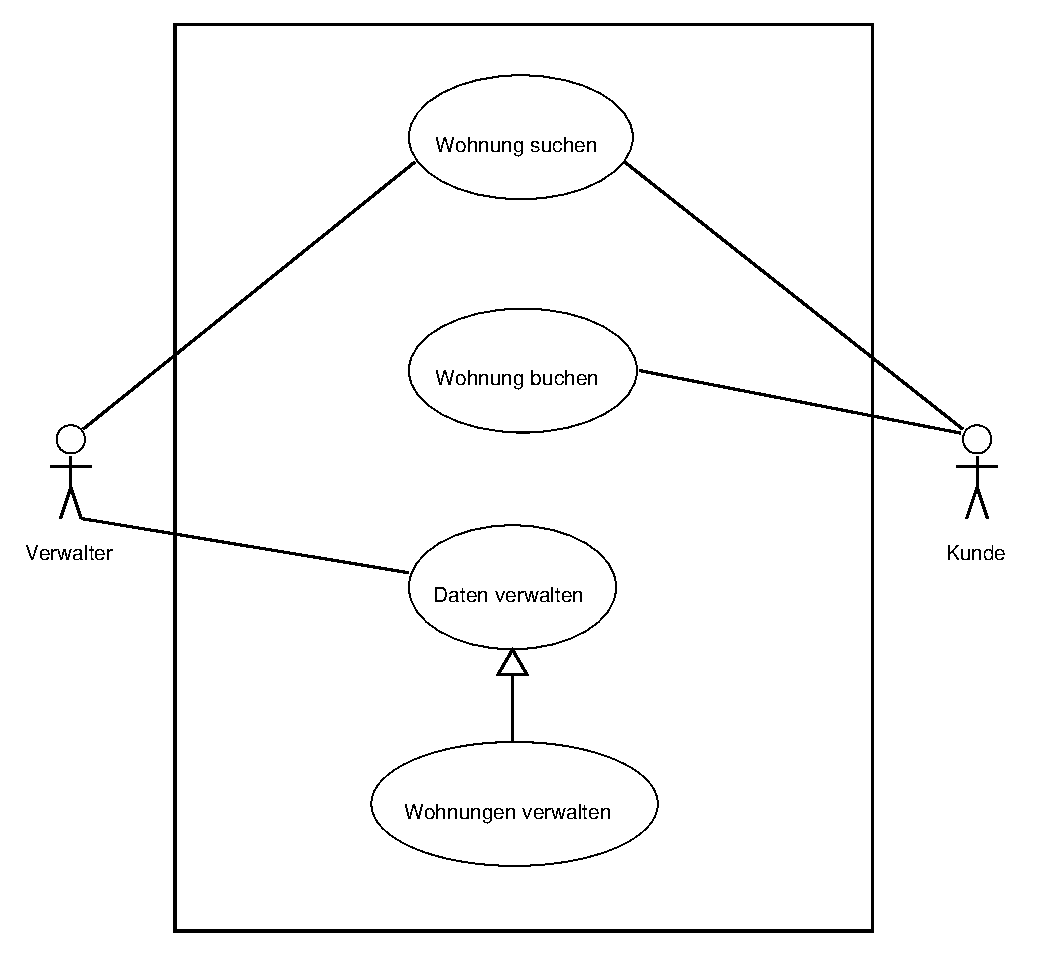
\includegraphics[width=0.90\textwidth]{images/beispielapplikation-anwendungsfaelle.eps}
	\caption{UML-Anwendungsfalldiagramm}
	\label{fig:beispielapplikation-anwendungsfaelle}
\end{figure}

\subsection{Suchen von Ferienwohnungen}
Dem Benutzer soll es erm�glicht werden, nach bestimmten Ferienwohnungen zu suchen. Dazu soll der Benutzer eine Eingabemaske angezeigt bekommen, in die er Suchkriterien eingeben kann. Diese Suchkriterien sind:
\begin{itemize}
	\item Land
	\item Anzahl der Zimmer
	\item Maximaler Preis
	\item Ausstattungsmerkmale
\end{itemize}
Die Ausgabe soll formatiert erfolgen. An die Formatierung werden keine besonderen Anforderungen gestellt.

Ziel des Nutzungsfalls ist die Suche nach alphanumerischen Werten �ber Joins (Suchkriterium Land). Die Joins sollen bei Oracle und SQL-Server �ber die Tabellen \texttt{Kunden} und \texttt{Wohnungen} erfolgen -- bei eXist �ber \acr{xml}-Dokumente. Dar�ber hinaus soll nach numerischen Werten (Suchkriterium Zimmer) und mit Vergleichsoperatoren wie kleiner/gr��er (Suchkriterium Preis) gesucht werden.

\subsection{Buchen von Ferienwohnungen}
Nachdem der Kunde eine Ferienwohnung gefunden hat, soll er die M�glichkeit haben, diese Wohnung zu buchen. Dazu soll der Benutzer das gew�nschte Anfangs- und Enddatum eingeben oder �ber ein Listenfeld ausw�hlen k�nnen. Die Buchung erfolgt �ber einen Klick auf eine Schaltfl�che. Anschlie�end soll die Software �berpr�fen, ob die Wohnung im fraglichen Zeitraum frei ist. Wenn dies der Fall ist, wird die Wohnung gebucht, d.h. es wird ein neuer Datensatz f�r die Buchung in der Datenbank abgelegt. Schl�gt die Buchung fehl, wird eine Fehlermeldung ausgegeben und der Kunde kann nochmals versuchen eine Wohnung zu buchen.

Ziel des Nutzungsfalls ist es zu testen, ob ein neuer Datensatz eingef�gt werden kann. Au�erdem soll �berpr�ft werden, ob die Datumsfunktionen auf \acr{xml}-Daten angewendet werden k�nnen. 

\subsection{Hinzuf�gen, �ndern und L�schen von Ferienwohnungen}
Die Firma soll in der Lage sein, neue Ferienwohnungen hinzuzuf�gen, zu l�schen oder zu �ndern. Das Hinzuf�gen erfolgt �ber eine einfache Eingabemaske, die nur aus Eingabefeldern besteht. Nach dem Beenden der Eingabe soll der Anwender durch Anklicken einer Schaltfl�che "`Hinzuf�gen"' die Eingabe best�tigen.

Beim L�schen sucht der Anwender zun�chst eine Ferienwohnung, wie im Nutzungsfall "`Suchen von Ferienwohnungen"' beschrieben. Wenn diese gefunden wurde, kann der Benutzer die Ferienwohnung durch Klicken auf eine Schaltfl�che "`L�schen"' aus der Datenbank entfernen.  

Die Funktion "`�nderung"' �hnelt dem Hinzuf�gen eines Datensatzes, mit dem Unterschied, dass zun�chst ein Datensatz gesucht wird. Dies geschieht ebenfalls wie im Nutzungsfall "`Suchen von Ferienwohnungen"' beschrieben wurde. Nachdem der Datensatz gefunden ist, kann dessen Inhalt in Eingabefeldern ge�ndert und durch die Schaltfl�che "`Best�tigen"' gespeichert werden.

Es existieren zwei Ansichen: Eine f�r den Verwalter und eine f�r den Kunden. Nur in der Ansicht f�r den Verwalter lassen sich Ferienwohnungen �ndern, hinzuf�gen und l�schen. Bei der Ansicht f�r den Kunden fehlen diese Funktionen. 

Ziel dieses Nutzungsfalls ist es, Einf�ge-, L�sch- und �nderungsoperationen bei Datenbanken unter Benutzung der \acr{xml}-Funktionalit�ten zu testen.

\section{Datenstrukturen}
Nachfolgend sind die \acr{dtd}s f�r die Speicherung der \acr{xml}-Daten in eXist sowie die \texttt{CREATE TABLE}-Statements f�r Oracle und \acr{sql}-Server aufgef�hrt.

\subsection{eXist}
\lstinputlisting[language=XML,caption={DTD f�r Wohnungen},label=listing:dtd-wohnungen]{Kapitel/Fallbeispiele/wohnungen.dtd}
\lstinputlisting[language=XML,caption={DTD f�r L�nder},label=listing:dtd-l�nder]{Kapitel/Fallbeispiele/laender.dtd}
\lstinputlisting[language=XML,caption={DTD f�r Kunden},label=listing:dtd-kunden]{Kapitel/Fallbeispiele/kunden.dtd}
\lstinputlisting[language=XML,caption={DTD f�r Buchungen},label=listing:dtd-buchungen]{Kapitel/Fallbeispiele/buchungen.dtd}

\subsection{Oracle}
\lstinputlisting[language=SQLORA,caption={CREATE-TABLE-Statement Wohnungen, Oracle},label=listing:oracle-xml-create-table-wohnung]{Kapitel/Fallbeispiele/oracle-xml-create-table-wohnung.txt}
\lstinputlisting[language=SQLORA,caption={CREATE-TABLE-Statement L�nder, Oracle},label=listing:oracle-xml-create-table-land]{Kapitel/Fallbeispiele/oracle-xml-create-table-land.txt}
\lstinputlisting[language=SQLORA,caption={CREATE-TABLE-Statement Kunden, Oracle},label=listing:oracle-xml-create-table-kunde]{Kapitel/Fallbeispiele/oracle-xml-create-table-kunde.txt}
\lstinputlisting[language=SQLORA,caption={CREATE-TABLE-Statement Buchungen, Oracle},label=listing:oracle-xml-create-table-buchung]{Kapitel/Fallbeispiele/oracle-xml-create-table-buchung.txt}

\subsection{SQL-Server}
\lstinputlisting[language=SQL05,caption={CREATE-TABLE-Statement Wohnungen, SQL-Server},label=listing:sql-server-create-table-wohnung]{Kapitel/Fallbeispiele/sql-server-create-table-wohnung.txt}
\lstinputlisting[language=SQL05,caption={CREATE-TABLE-Statement L�nder, SQL-Server},label=listing:sql-server-create-table-land]{Kapitel/Fallbeispiele/sql-server-create-table-land.txt}
\lstinputlisting[language=SQL05,caption={CREATE-TABLE-Statement Kunden, SQL-Server},label=listing:sql-server-create-table-kunde]{Kapitel/Fallbeispiele/sql-server-create-table-kunde.txt}
\lstinputlisting[language=SQL05,caption={CREATE-TABLE-Statement Buchungen, SQL-Server},label=listing:sql-server-create-table-buchung]{Kapitel/Fallbeispiele/sql-server-create-table-buchung.txt}

\section{Realisierung}
Die Realisierung der Anwendung erfolgt mittels der frei verf�gbaren Skriptsprache \acr{php} in der Version 5. Diese Sprache eignet sich besonders gut f�r den Einsatz bei Webapplikationen und es lassen sich relativ schnell Anwendungen erstellen, die �ber einen Webbrowser bedienbar sind. Ein weiterer Vorteil ist die Verf�gbarkeit einer ganzen Reihe von Standard-Klassen, die \zB einen einheitlichen Zugriff auf Datenbanksysteme erm�glichen.

Neben den verwendeten \acr{dbms} kommen also die folgenden Komponenten zum Einsatz:

\begin{itemize}
	\item Apache Webserver (Version 2.0.x) \footnote{\url{http://httpd.apache.org}}
	\item Skriptsprache \acr{php} (Version 5.x) \footnote{\url{http://www.php.net}}
	\item \acr{pear}-Datenbankabstraktionslayer "`DB"' \footnote{\url{http://pear.php.net/package/DB/}} -- erm�glicht Zugriff auf Oracle sowie Microsoft SQL-Server �ber die entsprechenden \acr{php}-Schnittstellen
	\item \acr{pear}-\acr{http}-Utilities "`HTTP"' \footnote{\url{http://pear.php.net/package/HTTP/}} -- komfortable Benutzung von \acr{http}-""Anfragen; dient der Ansteuerung von eXist.
	\item \acr{odbtp} -- Middleware f�r den \acr{sql}-Server
	\item die Ausgabe der Daten wird serverseitig �ber \acr{xsl}-Transformationssheets erstellt und durch den Webbrowser �ber \acr{css} formatiert dargestellt.
\end{itemize}

Neben diesen bereits verf�gbaren Standard-Komponenten spricht besonders die umfangreiche und einfach zu benutzende \acr{xml}-Unterst�zung f�r einen Einsatz von \acr{php}. Gerade in der aktuellen Version 5 wurden diese Funktionen komplett �berarbeitet und erweitert.

So gibt es neben der Unterst�tzung f�r \acr{sax}-Parsing und einem stark vereinfachten Interface f�r den Lese- und Schreibzugriff auf \acr{xml}-Dokumente (genannt "`simplexml"') auch eine Implementierung des \acr{w3c}-\acr{dom}-""Standards.

Weitere wichtige Bestandteile sind Schema-Validierung (\acr{dtd} und \acr{xsd}), Zugriff auf Dokumente per XPath sowie \acr{xsl}-Transformationen. Ebendiese \acr{xsl}-""Unterst�tzung wird in der Beispiel-Applikation f�r die dynamische Transformation der \acr{xml}-Daten in \acr{xhtml} verwendet.

\chapter{Umsetzung mit Oracle 9i}
\section{XML-Unterst�tzung}

F�r die Unterst�tzung von \acr{xml} bietet Oracle eine Reihe von Tools an. Diese Tools sind (Quelle: \citep{url:OracleXMLFAQ}):
\begin{itemize}
	\item XMLDB oder kurz XDB: Beinhaltet die mit Oracle 9i (oder sp�tere Versionen) standardm��ig ausgelieferte \acr{xml}-Unterst�tzung.
	\item \acr{xml}-\acr{sql}-Utility (XSU): Interfaces f�r die Programmiersprachen \acr{plsql} und Java.
	\item \acr{xml}-Developer Kit (XDK):  Es bietet eine Reihe von Tools f�r die Schnittstelle von \acr{xml} und Oracle. Es bietet Unterst�tzung f�r C, C++, Java und \acr{plsql}.
	\item XSQL Servlet: Erm�glicht die dynamische Generierung von \acr{xml}-""Dokumenten.
	\item weitere Tools wie beispielsweise Oracle iFS, Oracle InterMedia, JDeveloper.
\end{itemize}

F�r das Projekt wurde nur XDB benutzt. Die �brigen Tools werden deshalb und aus Zeitgr�nden hier nicht n�her betrachtet.

\section{Unterstz�tzung des SQL/XML-Standards}
Wie es der \acr{sql}/\acr{xml}-Standard vorschreibt, lassen sich relationale Daten mit \acr{xml}-Daten kombinieren. Der Datentyp wird bei Oracle allerdings als \texttt{XMLType} bezeichnet und nicht als \texttt{XML} wie im Standard vorgeschrieben \citep{Tuerker2003}.

Der \acr{sql}/\acr{xml}-Standard ist noch nicht vollst�ndig umgesetzt. In Oracle 9i werden nur die folgenden Elemente des Standards unterst�tzt:
\begin{itemize}
	\item \texttt{XMLAgg()}
	\item \texttt{XMLConcat()}
	\item \texttt{XMLElement()}
	\item \texttt{XMLForest()}
\end{itemize}

In sp�teren Versionen ist laut Oracle eine vollst�ndige Unterst�tzung des Standards geplant (Quelle: \citep{url:oracleTechnologyXML}).

Neben dem im \acr{xml}-Standard beschriebenen Funktionen besitzt Oracle weitere Funktionen f�r die \acr{xml}-Unterst�tzung. Dies sind unter anderem:

\begin{itemize}
	\item \texttt{SYS\_XMLGEN()}: Die Funktion ist �hnlich der Funktion \texttt{XMLElement()}. Der einzige Unterschied besteht darin, dass die Funktion nur ein einziges Attribut aufnehmen kann und dieses in \acr{xml} umwandelt.
	\item \texttt{SYS\_XMLLAGG()}: Aggregiert alle Elemente eines \acr{xml}-Dokuments oder ein Fragment davon und erzeugt ein \acr{xml}-Dokument. Das daraus entstehende Dokument wird in einem Element mit dem Defaultnamen "`ROWSET"' eingeschlossen.
\end{itemize}

(Quelle: \citep{OracleSQL})

Es existieren eine Reihe von Methoden des Typs \texttt{XMLType}. Die folgende Liste ist eine unvollst�ndige Aufz�hlung dieser Methoden, die auch im untersuchten Projekt benutzt werden:

\begin{itemize}
  \item \texttt{XMLType()}: Konstruktor zum Erzeugen einer \texttt{XMLType}-Instanz
	\item \texttt{updateXML()}: �nderung eines einzelnen \acr{xml}-Elements.
	\item \texttt{extract()}: Erm�glicht eine Abfrage mit XPath und liefert einen Teilbaum zur�ck.
	\item \texttt{existsNode()}: Pr�ft, ob ein Knoten existiert. Wenn der Knoten vorhanden ist, so wird eine 1 zur�ckgeliefert, andernfalls eine 0.
	\item \texttt{getClobVal()}: Liefert den Wert einer \texttt{XMLType}-Instanz als \acr{clob}-Wert zur�ck.
	\item \texttt{getStringVal()}: Liefert den Wert einer \texttt{XMLType}-Instanz als Zeichenkette zur�ck.
	\item \texttt{getNumVal()}: Liefert den Wert einer \texttt{XMLType}-Instanz als numerischen Wert zur�ck.
\end{itemize}

\section{Unterst�tzung von XPath und XQuery}

Oracle unterst�tzt au�erdem XPath. Dazu stellt das Oracle-\acr{dbms} die Funktion \texttt{extract()} zur Verf�gung.

XQuery hingegen wird erst ab Version 10i weitestgehend unterst�tzt. (Quelle: \citep{url:oracleXQuery})

\chapter{Umsetzung mit Microsoft SQL-Server}
\section{Einleitung}
Das Testsystem l�uft mit der Version 2005 "`June Community Technology Preview Readiness Kit"' von Microsoft. Die Anfragen und Ergebnisse werden �ber eine Middleware namens \acr{odbtp}\footnote{\url{http://odbtp.sourceforge.net}} versendet bzw. empfangen. Dies erst erm�glicht uns die Verarbeitung mit dem \acr{xml}-Datentyp. Mit den bereitgestellten \acr{php}-Funktionen war dies vorher nicht m�glich.

\section{Erstellung von Indexen}
Die XQuery-Abfragen k�nnen mit einem prim�ren und sekund�ren Index optimiert werden. F�r die Tabelle Wohnung sieht das folgenderma�en aus:
\lstinputlisting[language=SQL05,caption={SQL XML prim�rer Index},label=listing:sql-server-index-primar]{Kapitel/Fallbeispiele/sql-server-xml-index-primar.txt}
\lstinputlisting[language=SQL05,caption={SQL XML sekund�rer Index},label=listing:sql-server-index-sekundar]{Kapitel/Fallbeispiele/sql-server-xml-index-sekundar.txt}

Weitere Informationen dazu unter Kapitel \ref{sql-server-xml-index}.

\section{Abfragetypen}
\subsection{Suchen von Ferienwohnungen}

Suchen von Ferienwohnungen erfolgt im Fallbeispiel folgenderma�en:
\lstinputlisting[language=SQL05,caption={SQL-Server Suchen von Ferienwohnungen},label=listing:sql-server-su-ferienw]{Kapitel/Fallbeispiele/sql-server-wohnung-suchen.txt}

In der SELECT-Anweisung weisen wir in der \emph{FOR XML PATH}-Syntax die Spalten den gew�nschten Element- bzw. Attributnamen zu. Da der \acr{xml}-Datentyp in der Spalte \texttt{ausstattung} bereits \acr{xml}-Fragmente enth�lt, m�ssen mit dem Wildcard \texttt{*} die \acr{xml}-Daten direkt in das Ergebnis-Dokument eingef�gt werden.

\newpage
\subsection{Buchen von Ferienwohnungen}
\lstinputlisting[language=SQL05,caption={SQL-Server Buchen von Ferienwohnungen},label=listing:sql-server-bu-ferienw]{Kapitel/Fallbeispiele/sql-server-wohnung-buchen.txt}

Beim Buchen einer Ferienwohnung selektiert man im \acr{xml}-Feld \texttt{zeitraum} mit der XQuery-Funktion \texttt{value()} einen Wert und konvertiert ihn in den Typ \emph{VARCHAR}. Mit \texttt{CAST()} konvertiert der SQL-Server den Text in ein Datumsformat. Die Datumsfunktionen von XQuery werden in der von uns verwendeten Version 2005 noch nicht unterst�tzt.

\subsection{Hinzuf�gen von Ferienwohnungen}
\lstinputlisting[language=SQL05,caption={SQL-Server Einf�gen einer Ferienwohnung},label=listing:sql-server-einf-ferienw]{Kapitel/Fallbeispiele/sql-server-wohnung-einfuegen.txt}

Die Daten in die Datenbank zu speichern erreichen wir mit einem einfachen \texttt{INSERT}-Befehl. Falls das \acr{xml}-Dokument als Datei vorliegt, ist es �ber \emph{OpenXML} m�glich, die Daten zu importieren. Dies wird in der folgenden Form am Beispiel des \acr{xml}-Dokuments "`L�nder"' umgesetzt:
\lstinputlisting[language=SQL05,caption={SQL-Server OpenXML},label=listing:sql-server-openxml]{Kapitel/Fallbeispiele/sql-server-openxml.txt}

Das \acr{xml}-Dokument wird in diesem Fall direkt eingef�gt und darf den Speicher von 8000 Zeichen nicht �berschreiten. Um gr��ere \acr{xml}-Dokumente in die Datenbank einzulesen, k�nnte das \acr{com} Objekt \emph{Bulk Load} (\citep{url:SQLSERV05_BULK_LOAD}) verwendet werden. Mit einer Programmiersprache wie \acr{php} ist es m�glich, auf diese \acr{com}-Schnittstelle (\citep{url:PHP_COM}) zuzugreifen und \acr{xml}-Daten in die Datenbank einzuf�gen. 

\subsection{�ndern von Ferienwohnungen}
\lstinputlisting[language=SQL05,caption={SQL-Server �ndern einer Ferienwohnung},label=listing:sql-server-bearb-ferienw]{Kapitel/Fallbeispiele/sql-server-update-ferienwohnung.txt}

Das Update erfolgt einfach durch �berschreiben der \acr{xml}-""Spalte \texttt{ausstattung}. Mit der XQuery-""Funktionen \texttt{modify()} w�re es m�glich, gezielt die \acr{xml}-Informationen zu bearbeiten.

\subsection{L�schen von Ferienwohnungen}
\lstinputlisting[language=SQL05,caption={SQL-Server L�schen einer Ferienwohnung},label=listing:sql-server-delete-ferienw]{Kapitel/Fallbeispiele/sql-server-delete.txt}
Anhand der ID des Datensatzes wird dieser aus der Datenbank gel�scht.

\section{Bewertung}
\subsection{Speicherung}
\begin{table}
	\sffamily
	\centering
	%\footnotesize
	\begin{tabularx}{\textwidth}{llX}
		\toprule
		
		\multicolumn{1}{@{}N}{Kriterium} & 
		\multicolumn{1}{@{}N}{Erf�llt?} & 
		\multicolumn{1}{@{}N}{Beschreibung} \\
		\midrule\addlinespace
		
		Unterst�tzte Speicherformen 			& 					& \acr{xml}-Dokument wird relational als \acr{xml}-Datentyp 
																										gespeichert, internes Format \acr{blob} \\ \cmidrule{1-3}
	  Komplette \acr{xml}-Dokumente 		& \ding{51} & ja, bis auf den Vorspann als \acr{xml}-Datentyp \\ \cmidrule{1-3}
	  Tabelle von \acr{xml}-Typ 				& \ding{55} & \textit{nicht zutreffend} \\ \cmidrule{1-3}
		Hybride Speicherung							 	& \ding{51} & ja, als \acr{xml} und relational \\ \cmidrule{1-3}	  
		\acr{sql}/\acr{xml}-Standard 			& \ding{55} & die \acr{xml}-Funktionen werden nicht unterst�tzt \\ 
								
		\addlinespace\bottomrule
		
  \end{tabularx}
	\caption{Bewertung: Speicherung}
	\label{tab:sql-server-bewertung-speicherung}
\end{table}

Wie in Tabelle \ref{tab:sql-server-bewertung-speicherung} beschrieben ist es m�glich, komplette \acr{xml}-Dokumente zu speichern. Jedoch mit der Einschr�nkung, dass der Vorspann gel�scht wird. Mit dem Datentyp \texttt{NVARCHAR} oder \texttt{VARBINARY} ist es m�glich, vollst�ndige \acr{xml}-Dokumente zu speichern. Indexe oder XQuery-Funktionen k�nnen darauf nicht angewendet werden.

\subsection{Abfragen}

\begin{table}
	\sffamily
	\centering
	%\footnotesize
	\begin{tabularx}{\textwidth}{llX}
		\toprule
		
		\multicolumn{1}{@{}N}{Kriterium} & 
		\multicolumn{1}{@{}N}{Erf�llt?} & 
		\multicolumn{1}{@{}N}{Beschreibung} \\
		\midrule\addlinespace
		
		XPath 									& \ding{51} & XPath 2.0, \acr{w3c} Working Draft aus dem November 2003. Standard-Funktionen nicht vollst�ndig implementiert. \\ \cmidrule{1-3}
	  XQuery 									& \ding{51} & XQuery 1.0, \acr{w3c} Working Draft aus dem November 2003. Standard-Funktionen nicht vollst�ndig implementiert. \\ \cmidrule{1-3}
	  �nderungsoperationen		& \ding{51}	& Mittels \texttt{modify()} und den XQuery-Funktionen (insert, delete, into, after, before, usw.). \acr{xml}-Daten werden auf Wohlgeformtheit hin �berpr�ft. \\ \cmidrule{1-3}
		Ergebnis-Darstellung		&  					& Mit \emph{FOR XML} R�ckgabe des \acr{xml}-Dokuments als String. \\ \cmidrule{1-3}
		Transaktionssicherheit	& \ding{51}	& Unterst�tzt werden Transaktionssicherheiten (\citep{url:SQLSERV05_XML_BEST_PRAC05}) auf Spalten mit dem \acr{xml}-Datentyp \\
								
		\addlinespace\bottomrule
		
  \end{tabularx}
	\caption{Bewertung: Abfragen}
	\label{tab:sql-server-bewertung-abfragen}
\end{table}

Wie in der Tabelle \ref{tab:sql-server-bewertung-abfragen} beschrieben, sind die XPath- und XQuery-Funktionen nicht vollst�ndig implementiert. Die im Fallbeispiel verwendete Datenbankversion 2005 ist nicht auf dem aktuellsten Stand der Entwicklung. Welche Funktionen in der endg�ltigen Version implementiert werden, ist zum Zeitpunkt der Erstellung dieser Studienarbeit noch offen. Weitere Informationen dazu unter Kapitel \ref{einschraenkungen-und-aktuelle-entwicklungen} und \citep{url:SQLSERV05_XQUERY}.

\subsection{Indexierung}
\begin{table}[H]
	\sffamily
	\centering
	%\footnotesize
	\begin{tabularx}{\textwidth}{llX}
		\toprule
		
		\multicolumn{1}{@{}N}{Kriterium} & 
		\multicolumn{1}{@{}N}{Erf�llt?} & 
		\multicolumn{1}{@{}N}{Beschreibung} \\
		\midrule\addlinespace
		
		Elemente	& \ding{51} & wird unterst�tzt mit dem sekund�ren \emph{PATH}-Index \\ \cmidrule{1-3}
	  Attribute	& \ding{51} & wird unterst�tzt mit dem sekund�ren \emph{PROPERTY}-Index und \emph{VALUE}-Index \\ \cmidrule{1-3}
	  Text			& \ding{51} & wird unterst�tzt mit dem prim�ren Volltextindex \\ 
								
		\addlinespace\bottomrule
		
  \end{tabularx}
	\caption{Bewertung: Indexierung}
	\label{tab:sql-server-bewertung-indexierung}
\end{table}

Die Indexe k�nnen Zugriffe mittels XQuery-Funktionen auf die \acr{xml}-Felder beschleunigen. Genauere Informationen dazu unter Kap. \ref{sql-server-xml-index} und \citep{url:SQLSERV05_XML_INDEX}.

\chapter{Umsetzung mit eXist}
\section{Einf�hrung in eXist}
eXist ist eine unter der \acr{gnu} \acr{lgpl} Open Source-Lizenz ver�ffentlichte native \acr{xml}-Datenbank \citep{url:Meier2005b}. Sie ist in Java implementiert und speichert die Daten in einem propriet�ren, vom dbXML-Projekt\footnote{\url{http://www.sleepycat.com/products/bdbxml.html}} abgeleiteten Format.

F�r die Abfrage von Daten werden die \acr{w3c}-Standards XPath 2.0 sowie XQuery 1.0 (erweitert um einige spezielle Funktionen und Operatoren) unterst�tzt. Zugriff auf die Datenbank ist �ber \acr{http}/\acr{rest}, \acr{xml-rpc}, \acr{soap} sowie das Java-\acr{xml}:DB-\acr{api} m�glich. Au�erdem sind �ber XUpdate sowie (auf dem Entwurf von \citep{Lehti2001} basierenden) XQuery-Erweiterungen Manipulationen auf Dokumenten- und Knoten-Ebene durchf�hrbar. Weitere technische Details finden sich auf der entsprechenden Webseite des Projekts \citep{url:Meier}.

Obwohl es derzeit noch einige Einschr�nkungen gibt, die einen Einsatz im professionellen High-End-Bereich nicht empfehlenswert machen w�rden, bietet eXist bereits zahlreiche gute Features und eine f�r kleinere Anwendungen ausreichende Performanz.

F�r die Evaluierung in dieser Arbeit wird eine aktuelle Entwicklungsversion vom 06.01.2006 verwendet.

\section{Funktionsweise}
In den folgenden Abschnitten soll die Funktionsweise der einzelnen Komponenten kurz beschrieben werden.

\subsection{Datenspeicherung}
Intern werden Dokumente in sog. \emph{Collections} (entsprechen dem "`Datenbank"'-""Konzept bei relationalen \acr{dbms}) zusammengefasst. Diese Collections k�nnen wiederum andere Collections enthalten, dadurch entsteht eine hierarchische, dateisystem�hnliche Struktur der Dokumente.

Die Datenablage erfolgt auf der Basis von \emph{B+-B�umen}. Diese Datenstruktur bietet aufgrund ihrer Selbst-Balanciertheit eine garantierte obere Schranke f�r die Operationen \emph{Suchen}, \emph{Einf�gen} sowie \emph{L�schen} (s. \citep{url:Papakonstantinou1999}). Besonders vorteilhaft ist die Verwendung der B-B�ume f�r die Verwaltung von gro�en Datenmengen, die evtl. teilweise in einen Hintergrundspeicher ausgelagert werden m�ssen -- insbesondere die gew�hlte Sonderform der B+-B�ume minimiert die n�tigen (teuren) Zugriffe auf diesen Hintergrundspeicher (\zB eine Festplatte).

\subsection{Dokumenten-Parsing und Indexierung}
Zum Parsen der Dokumente verwendet eXist die bereits vorgestellte \acr{sax}, mithilfe derer eine interne Baum-Repr�sentation des Dokumentes erstellt wird. Der so erstellte Baum sowie evtl. vorhandene Namensraum-Definitionen werden in (nach Namensr�umen) getrennten Dateien abgelegt. 

Die Speicherung der verschiedenen Knoten-Typen wird dabei unterschiedlich gehandhabt:
\begin{itemize}
	\item Elemente sowie dazugeh�rige Attributnamen werden im \emph{Struktur-Index} abgelegt
	\item Attributwerte werden im \emph{Volltext-Index} gespeichert
	\item Der Inhalt von Text-Knoten wird ebenfalls im \emph{Volltext-Index} abgelegt
\end{itemize}

Neben den genannten Indizes verwaltet eXist weiterhin einen \emph{Bereichsindex}, der im Gegensatz zu den o.g. jedoch manuell angelegt werden muss. Der Bereichsindex wird dabei typspezifisch f�r einzelne Dokumenten-Knoten definiert.

\subsection{Abfrage-Auswertung}
Abfragen k�nnen an einzelne Dokumente oder auch komplette Collections gestellt werden. Dabei wird die Abfrage intern zun�chst auf eine Reihe von Grundoperationen (Un-/Gleichheit, Gr��envergleich, Mengenoperation) zur�ckgef�hrt, f�r welche die B-Baum-Implementierung Abfragefunktionen zur Verf�gung stellt.

Der Dokumenten-Baum wird nun rekursiv abgestiegen, dabei wird in jedem Rekursionsschritt die Menge der noch zu durchsuchenden Knoten soweit wie m�glich eingeschr�nkt. Bei Erreichen eines Blattes (in welchen die eigentlichen Daten referenziert sind), werden die dort gefundenen Werte mittels der entsprechenden Testfunktion �berpr�ft -- bei erfolgreichem Test wird der Wert in die Ergebnismenge �bernommen.

\section{Einschr�nkungen und aktuelle Entwicklungen}
Aufgrund der Tatsache, dass es sich bei eXist um ein kleines Open Source-Projekt handelt, sind einige wichtige Features noch nicht verf�gbar bzw. existieren noch einige Einschr�nkungen -- diese sind aber teilweise bereits Bestandteil der aktuellen Entwicklungsarbeit (s. \citep{url:Meier2005}).

\begin{itemize}
	\item Keine Unterst�tzung f�r \emph{Transaktionen}, Crash-Recovery, Journalling-Log (erste Ans�tze in der aktuellen Entwicklungsversion)
	\item Beschr�nkung der \emph{Dokumentenanzahl} auf $2^{31}$
	\item Beschr�nkung der \emph{XML-Knoten pro Dokument} auf $2^{63}$ (Ans�tze zur Umgehung dieses Limits in
 Diskussion)
	\item XQuery 1.0/XPath 2.0 - Spezifikationen noch nicht komplett implementiert (wird stetig erweitert)
	\item Keine Unterst�tzung f�r \emph{Trigger} (undokumentiert vorhanden in der aktuellen Entwicklungsversion)
\end{itemize}

\part{Ergebnisse}
\section{Testläufe mit initialer Konfiguration}
Ziel dieser ersten Testläufe war es, herauszufinden, inwieweit das Fehlerziel 
mit den gewählten Parametern erreicht werden kann. Es wurden dabei jeweils 10 
Testläufe mit identischen Parametern durchgeführt, um "`Zufallstreffer"' 
(Gewichts- und Biaswerte werden bei Initialisierung des Netzes zufällig 
vergeben) auszuschließen. Tabelle \ref{tbl:21-5-3-ergebnisse} zeigt einen
Überblick über diesen Testlauf.

\begin{table}
	\sffamily
	\centering
	\footnotesize
	\begin{tabular}{Nllc}
		\toprule
		\multicolumn{1}{@{}N}{Nr.} &
		\multicolumn{1}{V{3.5em}@{}}{Epoche} &
		\multicolumn{1}{V{3.5em}@{}}{MSE} &
		\multicolumn{1}{V{5em}@{}}{Ziel erreicht} \\
		\midrule\addlinespace

		1 & 781 & 3.239147e-003 & --- \\ \cmidrule(rl){1-4}
		2 & 268 & 3.237180e-003 & --- \\ \cmidrule(rl){1-4}
		3 & 2000 & 1.390480e-003 & --- \\ \cmidrule(rl){1-4}
		4 & 887 & 2.027749e-002 & --- \\ \cmidrule(rl){1-4}
		5 & 2000 & 1.708763e-003 & --- \\ \cmidrule(rl){1-4}
		6 & 664 & 1.756893e-002 & --- \\ \cmidrule(rl){1-4}
		7 & 1610 & 9.666874e-005 & $\checkmark$ \\ \cmidrule(rl){1-4}
		8 & 655 & 2.314696e-003 & --- \\ \cmidrule(rl){1-4}
		9 & 1737 & 1.851531e-003 & --- \\ \cmidrule(rl){1-4}
		10 & 338 & 3.238135e-003 & --- \\ 

		\addlinespace\bottomrule
		\end{tabular}
	\caption{Ergebnisse der Testreihe mit 21-5-3 Netz}
	\label{tbl:21-5-3-ergebnisse}
\end{table}

Lediglich ein Testlauf erreichte hier das Fehlerziel - die anderen brachen bei 
Erreichen der maximalen Epochenanzahl bzw. des minimalen Gradienten ab. 
Abbildung \ref{fig:plot-runs-1} zeigt beispielhaft den Verlauf der Performance 
(also des MSE) für Testlauf Nr. 1, Abbildung \ref{fig:plot-runs-7} zeigt den 
erfolgreichen Testlauf Nr. 7.

\begin{figure}
  \centering
  \subfloat[Testlauf Nr. 1: minimaler Gradient erreicht]{
    \label{fig:plot-runs-1}
    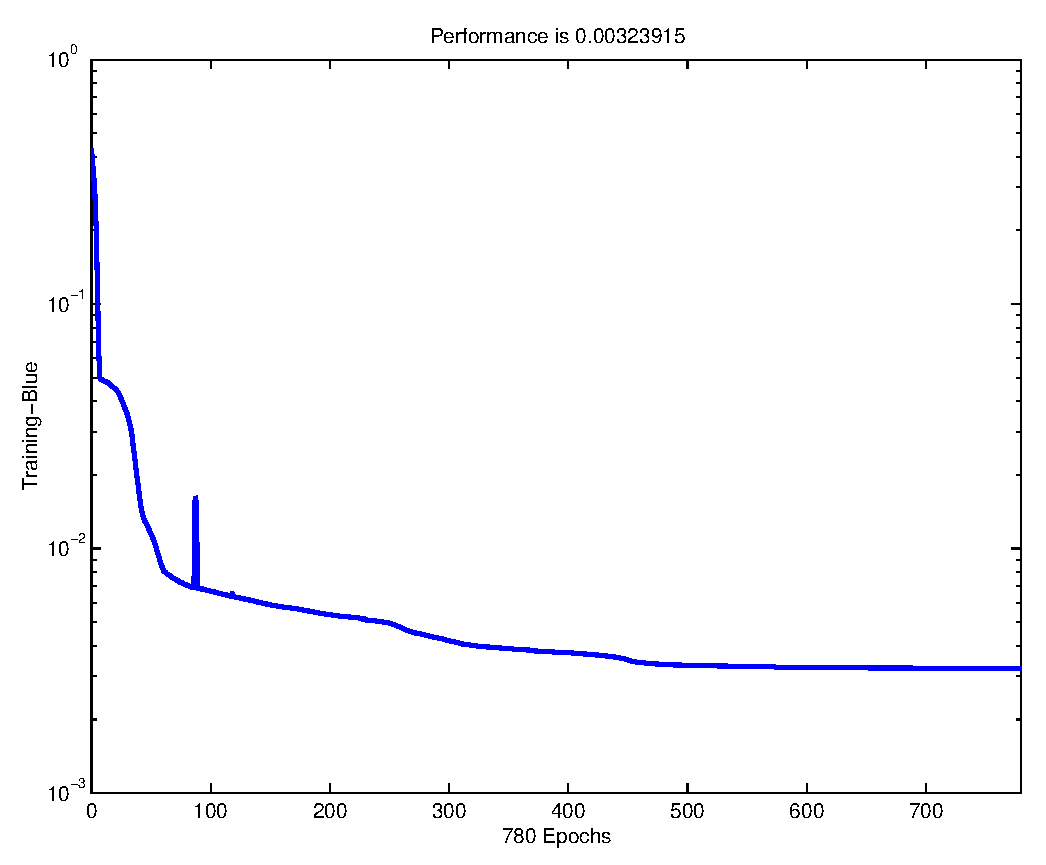
\includegraphics[width=0.45\textwidth]{../images/plots/21-5-3/21-5-3_1}
  }
  \subfloat[Testlauf Nr. 7: erfolgreich]{
    \label{fig:plot-runs-7}
    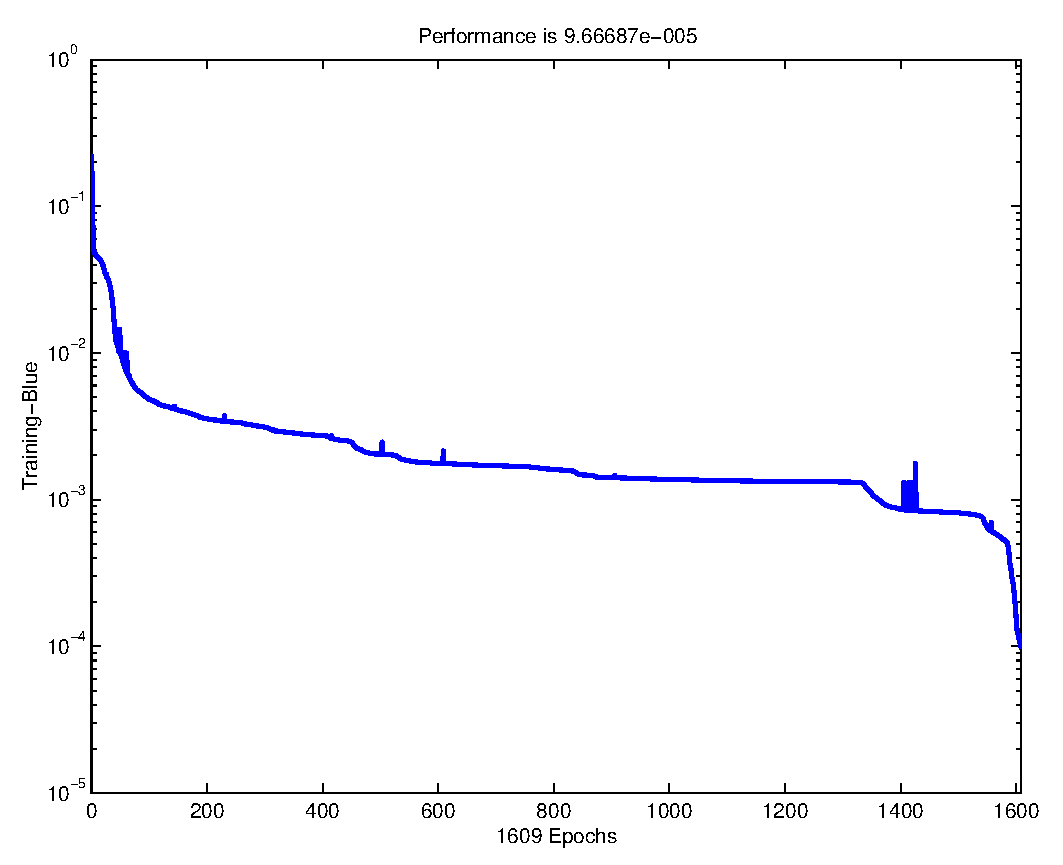
\includegraphics[width=0.45\textwidth]{../images/plots/21-5-3/21-5-3_7}
  }
  \caption{Verlauf der Performance zweier Testläufe}
  \label{fig:plot-runs}
\end{figure}

\section{Variation der Netzkonfiguration}
Wie im vorherigen Abschnitt zu sehen, erreichte das Netz mit nur 5 Neuronen in 
einer verdeckten Schicht das vorgegebene Fehlerziel (MSE) von $1 \cdot 10^{-4}$
lediglich in einem der Testläufe. Daher werden nun in einem ersten Schritt die
Anzahl der Neuronen in der verdeckten Schicht erhöht. Tabelle
\ref{tbl:var-neuronen} zeigt die Ergebnisse für diesen Versuch; in der letzten
Spalte ist aufgeführt, wie viele der 10 Testläufe das Fehlerziel erreicht haben. 

\begin{table}
	\sffamily
	\centering
	\footnotesize
	\begin{tabular}{lllc}
		\toprule
		\multicolumn{1}{V{7em}@{}}{Neuronen 1. verdeckte Schicht} &
		\multicolumn{1}{V{7em}@{}}{Epoche Durchschnitt} &
		\multicolumn{1}{V{7em}@{}}{MSE Durchschnitt} &
		\multicolumn{1}{V{5em}@{}}{Ziel erreicht} \\
		\midrule\addlinespace

		10 & 690 & 1.129535e-003 & 2/10 \\ \cmidrule(rl){1-4}
		15 & 473 & 1.222659e-003 & 2/10 \\ \cmidrule(rl){1-4}
		20 & 463 & 9.913476e-004 & 2/10 \\ \cmidrule(rl){1-4}
		25 & 391 & 8.526345e-004 & 2/10 \\ \cmidrule(rl){1-4}
		30 & 382 & 6.968107e-004 & 5/10 \\ \cmidrule(rl){1-4}
		35 & 382 & 6.957020e-004 & 5/10 \\ \cmidrule(rl){1-4}
		40 & 379 & 9.908886e-004 & 2/10 \\ \cmidrule(rl){1-4}
		45 & 380 & 1.195249e-003 & 4/10 \\ \cmidrule(rl){1-4}
		50 & 315 & 1.176323e-003 & 2/10 \\ 

		\addlinespace\bottomrule
		\end{tabular}
	\caption{Ergebnisse der Testreihe mit variierender Neuronenzahl}
	\label{tbl:var-neuronen}
\end{table}

Wie sich zeigt, wird das Fehlerziel in dem Netz mit \emph{einer} verdeckten Schicht 
maximal in 50\% der Testläufe erreicht. Es wird nun in einem weiteren Versuch 
mit einem Netz mit \emph{zwei} verdeckten Schichten gearbeitet. Auch hier wird wieder wie 
zuvor die Anzahl der Neuronen variiert und mit jeweils 10 Testläufen 
gearbeitet. Es werden hier nur die vielversprechendsten Kombinationen getestet;
Tabelle \ref{tbl:var-schichten} zeigt die Ergebnisse.

\begin{table}
	\sffamily
	\centering
	\footnotesize
	\begin{tabular}{llllc}
		\toprule
		\multicolumn{1}{V{7em}@{}}{Neuronen 1. verdeckte Schicht} &
		\multicolumn{1}{V{7em}@{}}{Neuronen 2. verdeckte Schicht} &
		\multicolumn{1}{V{7em}@{}}{Epoche Durchschnitt} &
		\multicolumn{1}{V{7em}@{}}{MSE Durchschnitt} &
		\multicolumn{1}{V{5em}@{}}{Ziel erreicht} \\
		\midrule\addlinespace

		10 & 10 & 328 & 1.581422e-003 & 1/10 \\ \cmidrule(rl){1-5}
		15 & 15 & 327 & 5.940588e-004 & 4/10 \\ \cmidrule(rl){1-5}
		30 & 30 & 210 & 4.081598e-004 & 5/10 \\ \cmidrule(rl){1-5}
		35 & 35 & 215 & 4.459380e-004 & 4/10 \\ \cmidrule(rl){1-5}
		45 & 45 & 174 & 3.408588e-004 & 7/10 \\

		\addlinespace\bottomrule
		\end{tabular}
	\caption{Ergebnisse der Testreihe mit zwei verdeckten Schichten}
	\label{tbl:var-schichten}
\end{table}

Wie man den Testläufen entnehmen kann, scheint eine Netztopologie 21-45-45-3 am
besten mit dieser Auswahl von Trainigsdaten trainierbar. Daher wird für die
folgenden Simulationsversuche zunächst auf diese Konfiguration zurückgegriffen.

\section{Simulation des Netzes mit ermittelter Konfiguration}
Im ersten Versuch wird hier das Netz mit den verbleibenden Datensätzen 
simuliert, die nicht für das Training verwendet wurden. Dazu wird der folgende
Funktionsaufruf verwendet:

\begin{lstlisting}[numbers=none]
[ySim, pf, af, eSim, perf] = sim(net, simulationData');
\end{lstlisting}

Dabei wird zum einen das trainierte Netz \texttt{net} sowie die zur Simulation
zu verwendenden Daten übergeben. Die Simulation mit einem erfolgreich
trainierten Netz ergab die folgenden Ergebnise:

\begin{description}
  \item[Fehler Klasse 1:] 36/149, d.h. 75,84\% korrekt erkannt.
  \item[Fehler Klasse 2:] 68/331, d.h. 79,46\% korrekt erkannt.
  \item[Fehler Klasse 3:] 55/5999, d.h. 99,10\% korrekt erkannt.
  \item[Gesamtfehler:] 159/6479, d.h. 97,55\% korrekt erkannt.
\end{description}

Wie man sieht, wird in den Klassen 1 und 2 eine weitaus niedrigere 
Klassifikationsgüte erreicht als in Klasse 3. Dies ist auf die geringe Anzahl 
der Trainingsdaten zurückzuführen. Insgesamt erreichte das Netz mit 97,67\% 
jedoch schon ein recht gutes Ergebnis. Um die Generalisierungsfähigkeit des 
Netzes weiter zu steigern, wird nun versucht, die Anzahl der Trainingsdaten zu 
erhöhen. Es werden nicht mehr 10, sondern 50\% der Datensätze für das Training 
verwendet:

\begin{description}
  \item[Fehler Klasse 1:] 21/83, d.h. 74,70\% korrekt erkannt.
  \item[Fehler Klasse 2:] 22/184, d.h. 88,04\% korrekt erkannt.
  \item[Fehler Klasse 3:] 19/3333, d.h. 99,43\% korrekt erkannt.
  \item[Gesamtfehler:] 58/3600, d.h. 98,23\% korrekt erkannt.
\end{description}

Wie man sieht, kann die Klassifikationsgüte insgesamt durch die Erhöhung der
Anzahl der Trainingsdaten leicht verbessert werden. 

\section{Fazit}
Wie die vorangegangenen Versuche gezeigt haben, ist ein künstliches neuronales 
Netz eine fragiles Gebilde, welches von vielen Einflussfaktoren wie z.B. der Anzahl 
und Auswahl der Trainings- und Simulationsdaten beeinflusst wird. Auch die
Bestimmung der "`optimalen"' Netzkonfiguration ist nicht wirklich eindeutig,
sondern wurde hier hauptsächlich durch Testläufe und Intuition bestimmt. 

Insgesamt konnten im besten Fall ca. 98\% der Datensätze korrekt zugeordnet 
werden. Allerdings bleibt die Klassifikationsgüte für die Klassen 1 und 2 recht 
gering, was auf die relativ kleine Anzahl an zur Verfügung stehenden 
Datensätzen zurückzuführen ist. Für die Klassifikation in 
Schilddrüsenüberfunktion bzw. -unterfunktion ist das künstliche neuronale Netz 
also nur bedingt zu gebrauchen - bei der Entscheidung jedoch, ob ein Patient 
\emph{keine} Fehlfunktion hat, erzielt das Netz recht zuverlässige Ergebnisse.


%%%
%%% Anhaenge: Glossar, Bibliographie...
%%%

\cleardoublepage % oder \clearpage
\phantomsection 

\appendix
\pdfbookmark[-1]{\appendixname}{\appendixname} 

%%% Bibliographie-Stil
\bibliographystyle{dinat}

%%% Anstatt 'Literatur' -> 'Quellen'
\renewcommand{\bibname}{Quellenverzeichnis}

%%% Bibliographie ausgeben
\bibliography{Literatur}

%%% Glossar ausgeben
\printgloss{Glossar}

\end{document}
%%% END OF FILE